\chapter{Benthic Habitat Mapping}
\lhead{Benthic Habitat Mapping}
\label{BenthicHabitatMapping}
	
	 With the general theory and framework of Gaussian process inference provided in section \ref{Background:GaussianProcesses}, this chapter aims to extend such theory to the benthic habitat mapping context. In particular, specific classifier inference techniques are developed and built upon the existing Gaussian process classifier framework. This chapter focuses strictly on the inference techniques necessary for building a map of benthic habitats across a given region. The following chapter would then continue to build on such inference models for the purpose of informative seafloor exploration. 
	
	This thesis employs Gaussian process classifiers as the primary inference model for benthic habitat mapping. Gaussian processes are non-parametric, Bayesian models which is able to model a variety of phenomenon. They are known to allow the data to `speak for itself' and provide a principled inference framework for drawing conclusion regarding the gathered data \citep{GaussianProcessForMachineLearning}. 
	
	Figure \ref{Figure:InferenceFlow} visualises the information flow involved in a Gaussian process classifier, and describes the necessary inference stages involved for both habitat mapping and information inference, the latter of which allows informative exploration and is the focus of the next chapter.

	\begin{figure}[!htbp]
	\centering
		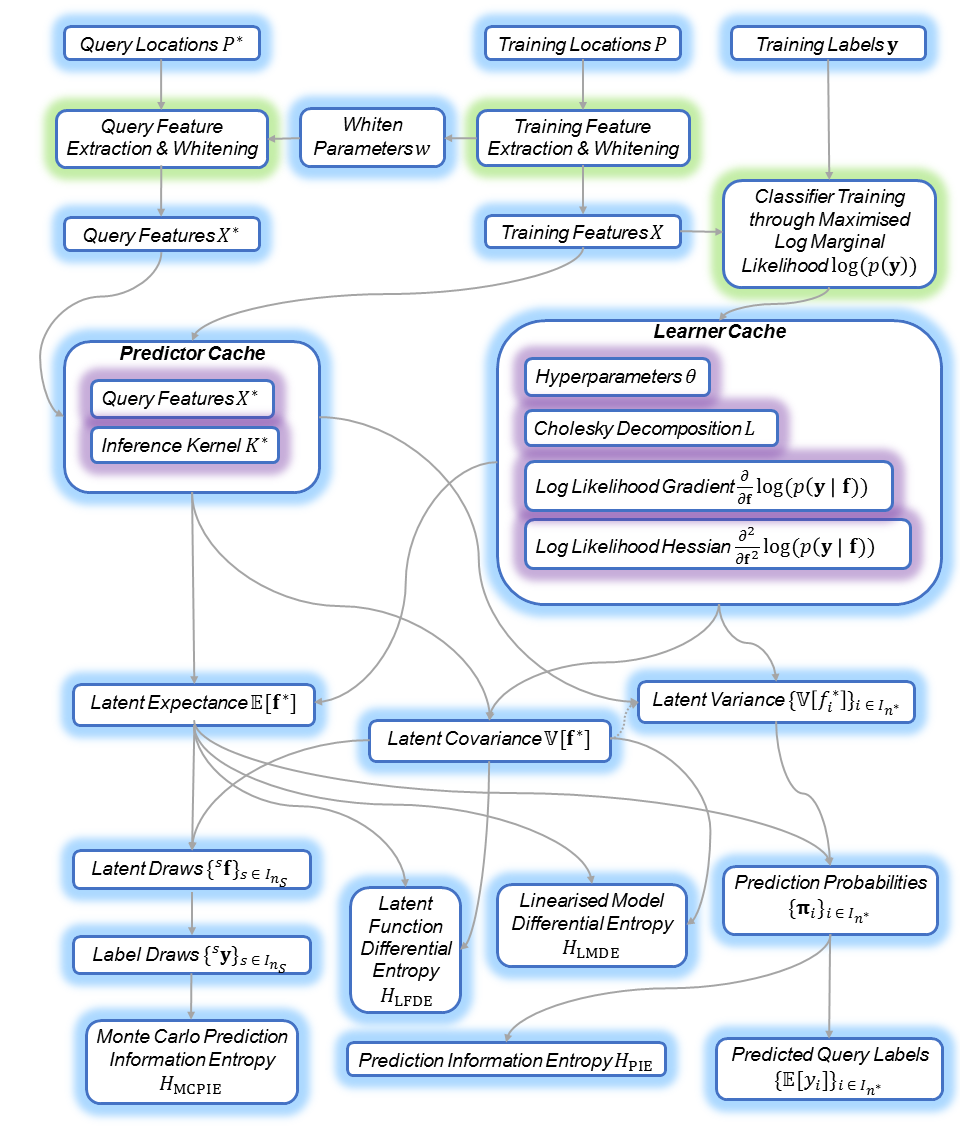
\includegraphics[width = 0.8\linewidth]{Figures/inferenceflow.eps}
	\caption{Inference Information Flow}
	\label{Figure:InferenceFlow}
	\end{figure}	
			
	This chapter will focus on the learning and inference stages represented by all the {\color{Gray} gray} and {\color{ForestGreen} green} coloured arrows, while the next chapter will focus on the inference stages represented by all the {\color{OrangeRed} red}, {\color{YellowOrange} gold}, and {\color{Cerulean} blue} coloured arrows.
	
	As the figure suggests, the mapping process is a supervised learning problem for which the habitat labels $\bvec{y}^{\star}$ at the query locations $P^{\star}$ is to be inferred from the query features $X^{\star}$ by learning a relationship between the habitat labels $\bvec{y}$ and the training features $X$ at the training locations $P$. Only the {\color{Gray} gray} and {\color{ForestGreen} green} coloured arrows in Figure \ref{Figure:InferenceFlow} are necessary for mapping to be achieved.
	
	As the discussion continues in the following two chapters, each part of the diagram will be expanded and addressed. The inference information flow provided in figure \ref{Figure:InferenceFlow} serves as a visual roadmap of the inference stages to be explored in this thesis, and will thus be reference frequently.
		
	 The benthic modeling process begins with extracting bathymetric features from given seafloor locations. Section \ref{BenthicHabitatMapping:BathymetricFeatures} discusses the process of bathymetric feature extraction which includes the modeling choices and assumptions involved, which covers {\color{BurntOrange} SPECIFY PARTS OF THE DIAGRAM BY COLOURED BUBBLES}. 
	 
	 (GP CHAPTERS DESCRIPTION)
	 
	 Finally, section \ref{BenthicHabitatMapping:ScottReef} demonstrates the techniques developed in this chapter through mapping the benthic habitats of the Scott Reef seafloor. 
		
	\section{Bathymetric Features}
	\label{BenthicHabitatMapping:BathymetricFeatures}
	
		This thesis can be broken down into two main parts - benthic habitat mapping and informative path planning. Benthic habitat mapping itself includes bathymetric feature extraction, and habitat class inference. Thus, benthic habitat mapping refers to the two stage process of feature extraction and habitat class inference, with the latter being the main bottleneck for this process. This section will focus on bathymetric feature extraction and modeling.
			
		In order for autonomous underwater vehicles to infer a map of the benthic habitats, and later plan a path to increase mapping accuracy, it would need a method to predict the types of environments it may encounter, with a measure of its prediction uncertainty.
		
		While the path planner is to plan in the spatial space, in general the prediction model operates upon some feature space with more direct and explicit relationships with the output to be inferenced.
		
		It is thus important to make a distinction between the feature space $\mathcal{X}$ for which benthic habitat modeling is to occur and the spatial space $\mathcal{P}$ for which bathymetric modeling and planning is to occur. The spatial space usually consists of Cartesian coordinates $(x, y)$ in the eastings-northings frame or the longitude-latitude frame, so that $\mathcal{P} \subseteq \mathbb{R}^{2}$. The path is to be planned in this spatial space. The frame is usually converted into a local body frame during the execution of control signals for path tracking. However, this does not affect the formulation presented here. The feature space $\mathcal{X} \subseteq \mathbb{R}^{p}$, where $p$ is the number of features (feature dimensions), includes bathymetric features for which the habitat labels will be modeled upon. Depending on the features employed for the modeling process, there are usually approximate analytical forms for extracting such features from raw depth observations.
		
		The following bathymetric features shown in \cref{Table:BathymetricFeatures} were selected for habitat mapping. The benthic habitats would be modelled upon five bathymetric features - bathymetric depth, aspect (short scale), rugosity (short scale), aspect (long scale), and rugosity (long scale). Spatial coordinates are chosen to be excluded from the bathymetric feature set. For benthic habitat mapping, it is expected that ecological habitats and geological sites exhibit no explicit relationship with the location of the site, and that its properties arise solely due to the local terrain structure and seafloor characteristics  of that site. This means that the nature of the habitat depends on the location implicitly through explicit dependence on bathymetric structure of the seafloor. These five bathymetric features summarises the local terrain structure at every location of the seafloor, and forms our feature space $\mathcal{X} \subseteq \mathbb{R}^{5}$ with $p = 5$.
		
		\begin{table}[h]
			\begin{center}
				\begin{tabular}{ l c c }
					\hline
					\hline
					Feature Name & Feature Symbol & Feature Units \\
					\hline
					\hline
					Depth & $z$ & m \\
					Aspect (Small Scale) & $a_{s}$ & m/m \\
					Aspect (Large Scale) & $a_{l}$& m/m \\
					Rugosity (Small Scale) & $r_{s}$ & $\mathrm{m^{2}/m^{2}}$ \\
					Rugosity (Large Scale) & $r_{l}$ & $\mathrm{m^{2}/m^{2}}$  \\
					\hline
					\hline
				\end{tabular}
			\end{center}
	  	\caption{Bathymetric Features}
	  	\label{Table:BathymetricFeatures}			
	  	\end{table}	
		
		Aspect also refers to the slope of the seafloor terrain, while rugosity is a measure of small-scale variations or amplitude in the height of a surface.
		
		The raw bathymetric data contains depth information at various spatial locations. Such data are often collected rather uniformly in approximate grid formations such that it is possible to calculate the ocean floor slope through finite differencing. The aspect, or slope, is divided into small scale and large scale variations, as marine environments - especially underwater habitats - often depend not only on the immediate slope but also slope variations on the larger scale. The same idea applies to rugosity to measure local height variations at two different scales.
		
		% Define block styles
		\tikzstyle{block} = [rectangle, draw, fill = green!10!blue!20, text width = 7.5em, text centered, rounded corners, minimum height = 4em]
		\tikzstyle{line} = [draw, -latex']
	
		\begin{figure}[!ht]
		\centering\makebox[\textwidth]{
			\begin{tikzpicture}[node distance =4cm, auto,
			comment/.style={
			rectangle, 
			inner sep= 5pt, 
			text width=4cm, }]
			
			\node [block] (spatialspace) {Seafloor Spatial Space $\mathcal{P}$};
			\node [block, right of = spatialspace] (featurespace) {Bathymetric Feature Space $\mathcal{X}$};
			\node [block, right of = featurespace] (mapspace) {Habitat Map Space $\mathcal{Y}$};
					
			\draw [line] (spatialspace) -- (featurespace);
			\draw [line] (featurespace) -- (mapspace);
			
			\draw [decorate ,decoration = {brace, amplitude = 10pt, raise = 3mm}]
			(spatialspace.85) -- (featurespace.95) node [black, midway, yshift = 10mm]
			{Bathymetric Feature Extraction};
			
			\draw [decorate, decoration = {brace, amplitude = 10pt, raise = 3mm}, xshift = 0pt, yshift = 0pt]
			(featurespace.85) -- (mapspace.95) node [black, midway, yshift = 6mm] 
			{Habitat Class Inference};
						
			\end{tikzpicture}}		
		\caption{Benthic Habitat Mapping Process}
		\label{Figure:BenthicHabitatMappingProcess}
		\end{figure}
		
		Figure \ref{Figure:BenthicHabitatMappingProcess} show a high level overview of the benthic habitat mapping process. As bathymetric data is available in more quantities and distributed more uniformly, it is often sufficient to employ the feature extraction process outlined in \cref{BenthicHabitatMapping:BathymetricFeatures:FeatureExtraction} to obtain the bathymetric features for modeling. However, if the bathymetric data is sufficiently sparse or is not distributed uniformly for grid based methods, then the feature extraction process itself becomes a prediction problem.

		In that case, a Gaussian process regression model is proposed for predicting the features at a given spatial location. While this is much more computationally expensive than performing feature extraction, it is also quite rare that this is necessary under abundant bathymetric data. In most cases, it suffices to simply take the nearest neighbouring feature.		
		
		\subsection{Formulation}
		
			With the basic structure of the benthic habitat mapping process presented above, the model spaces involved can now be formulated formally.
			
			As established previously, the spatial space $\mathcal{P} \subseteq \mathbb{R}^{2}$ and feature space $\mathcal{X} \subseteq \mathbb{R}^{5}$ are compact subsets of $\mathbb{R}^{2}$ and $\mathbb{R}^{5}$ respectively. On the other hand, the habitat map space $\mathcal{Y} \subset \mathbb{N}$ is a strict finite subset of the the natural numbers, with each distinct integer representing a particular habitat type.
			
			Further, define $\mathscr{P} := \mathscr{P}(\mathcal{P})$, $\mathscr{X} := \mathscr{X}(\mathcal{X})$, and $\mathscr{Y} := \mathscr{Y}(\mathcal{Y})$ as the $\sigma$-algebras generated by $\mathcal{P} \subseteq \mathbb{R}^{2}$, $\mathcal{X} \subseteq \mathbb{R}^{5}$, and $\mathcal{Y} \subset \mathbb{N}$ respectively. Specifically, this means that $X \in \mathscr{X}$ implies $X \subseteq \mathcal{X}$, and similarly for $\mathscr{P}$ and $\mathscr{Y}$.
			
			Note that if $X := \{\bvec{x}_{i}\}_{i \in I_{n}} := \{\bvec{x}_{1}, \bvec{x}_{2}, \dots, \bvec{x}_{n}\} \in \mathscr{X}$ is a \textit{finite} collection of feature vectors $\bvec{x}_{i} \in \mathcal{X}$ for all $i \in I_{n}$, then $X$ is equivalent to the matrix $[\bvec{x}_{1}, \bvec{x}_{2}, \dots, \bvec{x}_{n}]^{T} \in \mathbb{R}^{n \times p}$. For notational and analytical convenience, the two quantities will be considered equivalent such that $X := \{\bvec{x}_{i}\}_{i \in I_{n}} := \{\bvec{x}_{1}, \bvec{x}_{2}, \dots, \bvec{x}_{n}\} \equiv [\bvec{x}_{1}, \bvec{x}_{2}, \dots, \bvec{x}_{n}]^{T}$. This notation is used consistently throughout, and a similar formulation applies to spatial coordinates $P \in \mathscr{P}$. For target labels in the habitat map space, $\bvec{y} := \{y_{i}\}_{i \in I_{n}} := \{y_{1}, y_{2}, \dots, y_{n}\} \in \mathscr{Y}$ is already consistent with existing nomenclature for vectors, and also complies in form with the above matrix formulation. Recall that for an arbitrary quantity $q_{i}$ indexed by $i \in I_{n}$, $\{q_{i}\}_{i \in I_{n}}$ is defined to be $\{q_{1}, q_{2}, \dots, q_{n}\}$ which is equivalent to a vector if $q_{i}$ is a scalar and a matrix if $q_{i}$ is a vector.
		
		\subsection{Data Matching}
		\label{BenthicHabitatMapping:BathymetricFeatures:DataMatching}
		
			A subtlety that arises from the above formulation is that during the training stage, the bathymetric data and the label data are not necessarily observed at the same places. Figure \ref{Figure:ScottReefBathymetricFeatures} illustrates the spatial distribution of the two datasets in a typical setting using the Scott Reef data set \citep{IMOS} as an example. Note that the colour scales have been shifted to emphasize the feature variations.
		
			\begin{figure}[!htbp]
			\centering
			  \subfigure{\label{Figure:ScottReefBathymetricFeatures:1}	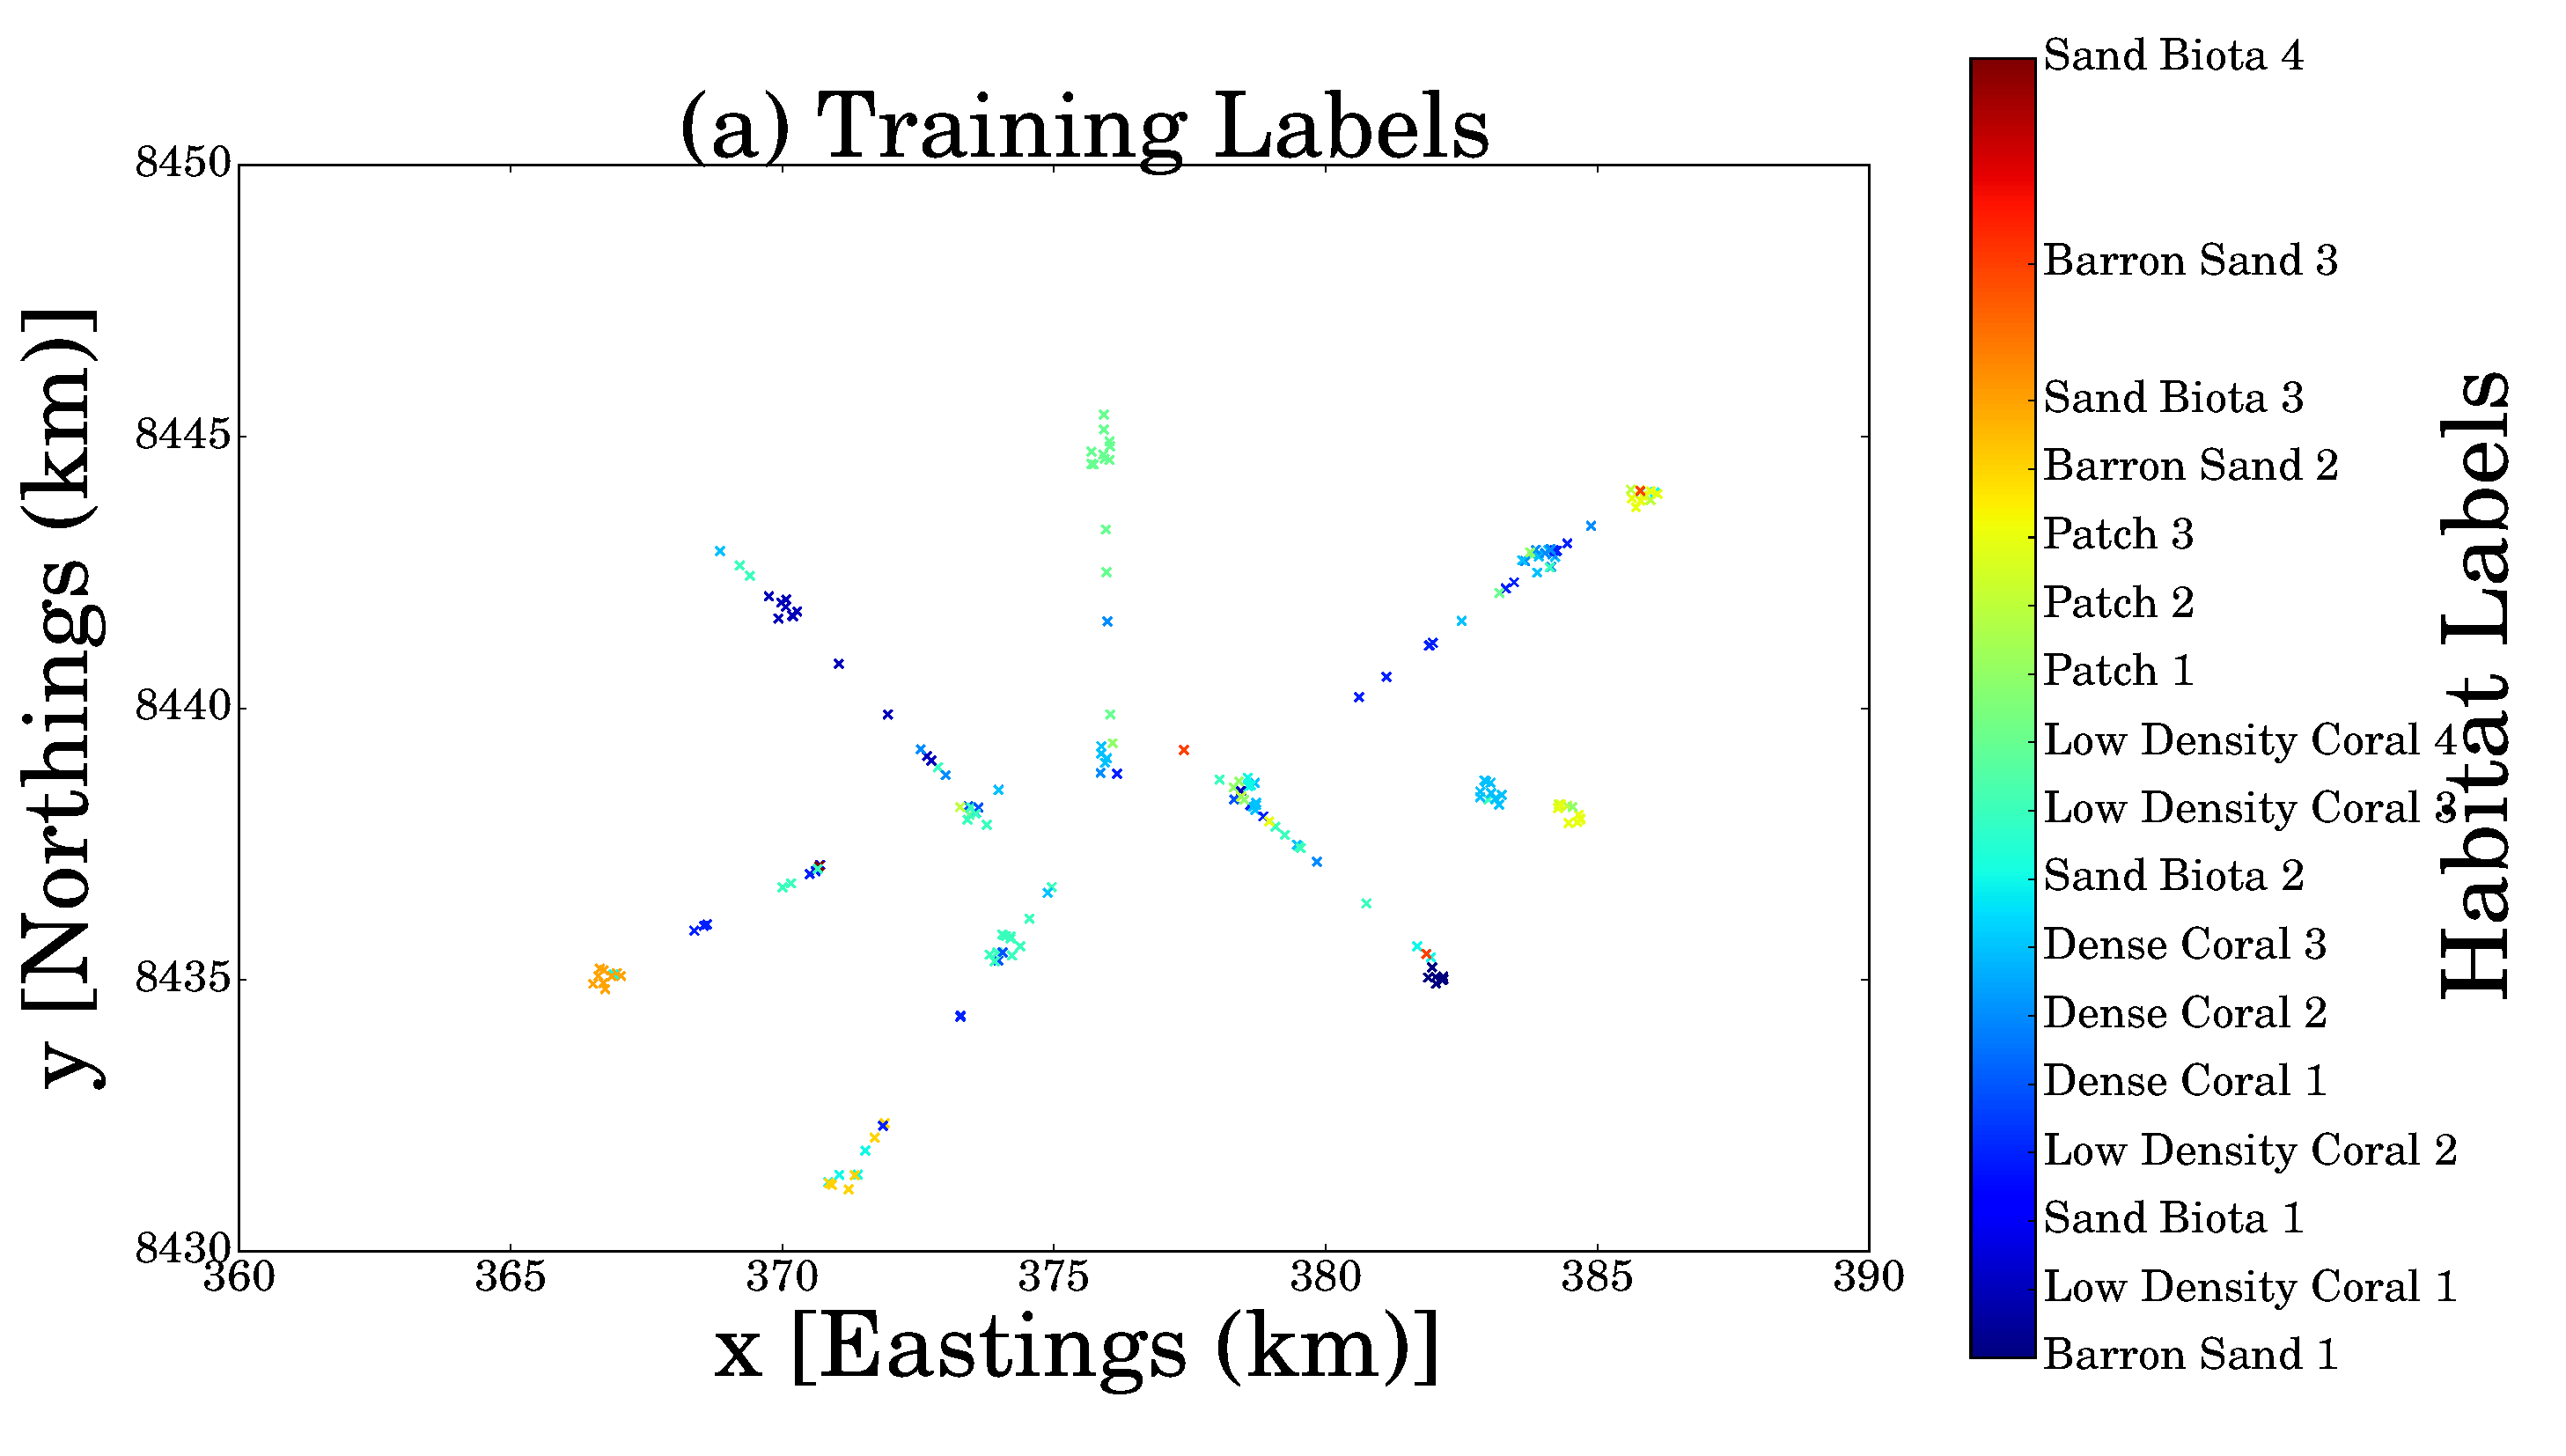
\includegraphics[width=0.48\linewidth]{Figures/scott_reef_mapping_one_colorbar/Figure1.eps}}
			  \subfigure{\label{Figure:ScottReefBathymetricFeatures:2}	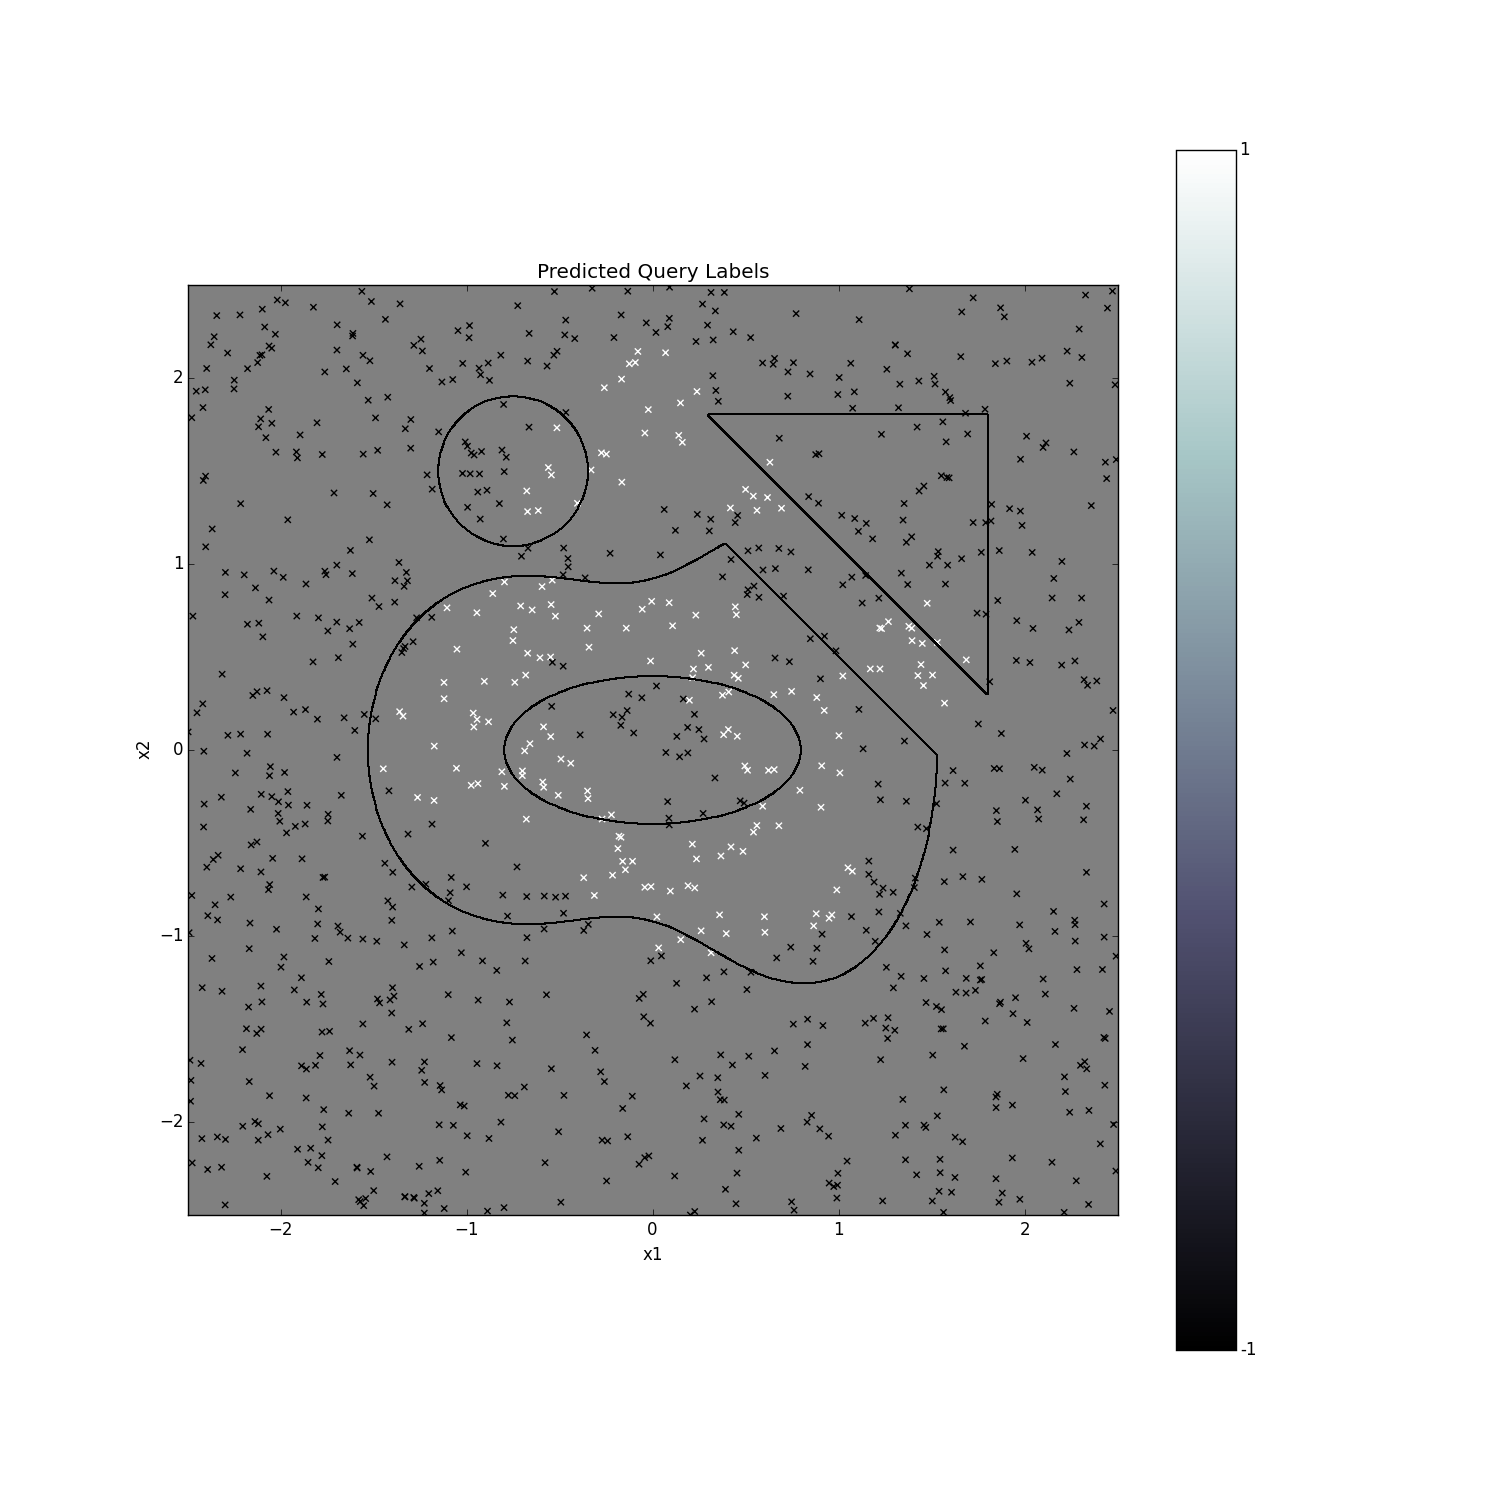
\includegraphics[width=0.48\linewidth]{Figures/scott_reef_mapping_one_colorbar/Figure2.eps}}
			  \subfigure{\label{Figure:ScottReefBathymetricFeatures:3}	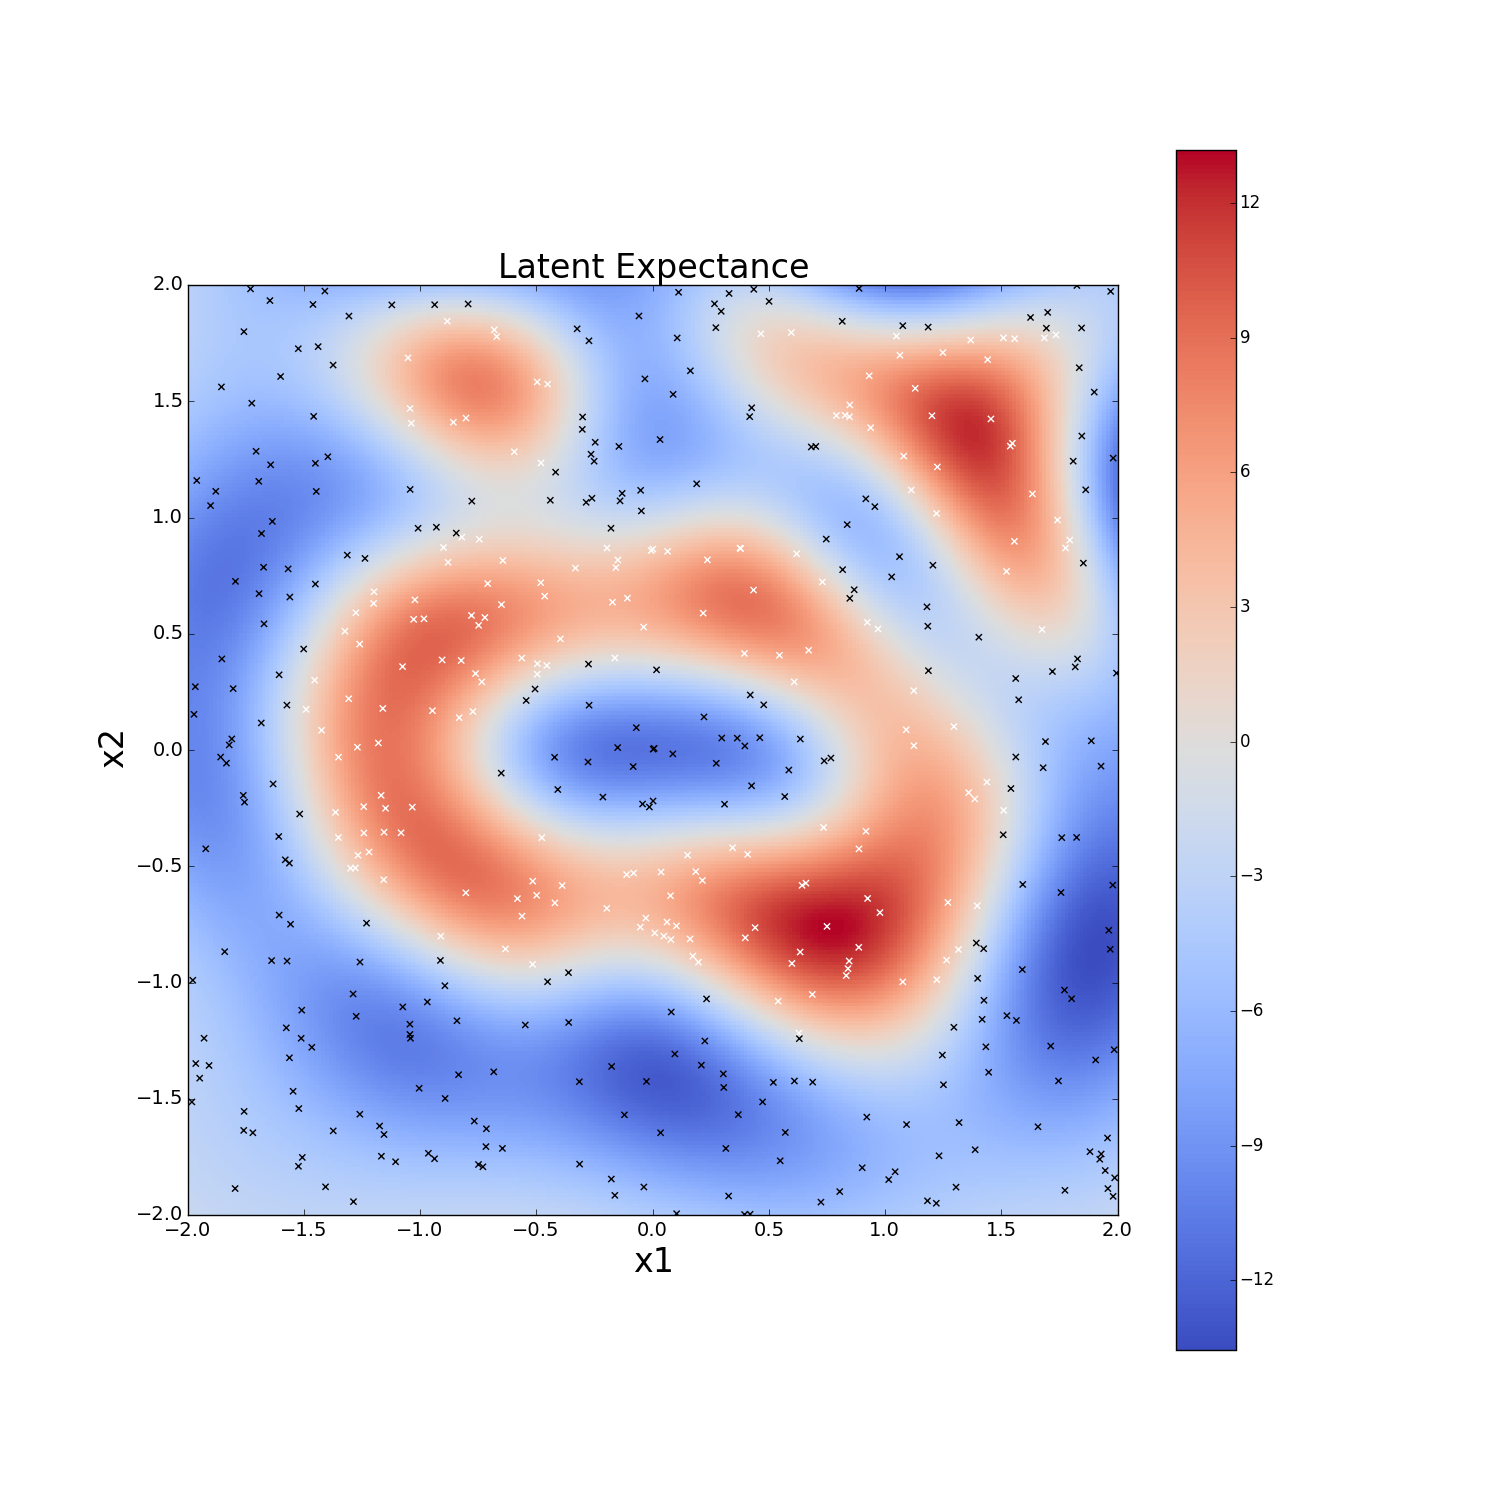
\includegraphics[width=0.48\linewidth]{Figures/scott_reef_mapping_one_colorbar/Figure3.eps}}
			  \subfigure{\label{Figure:ScottReefBathymetricFeatures:4}	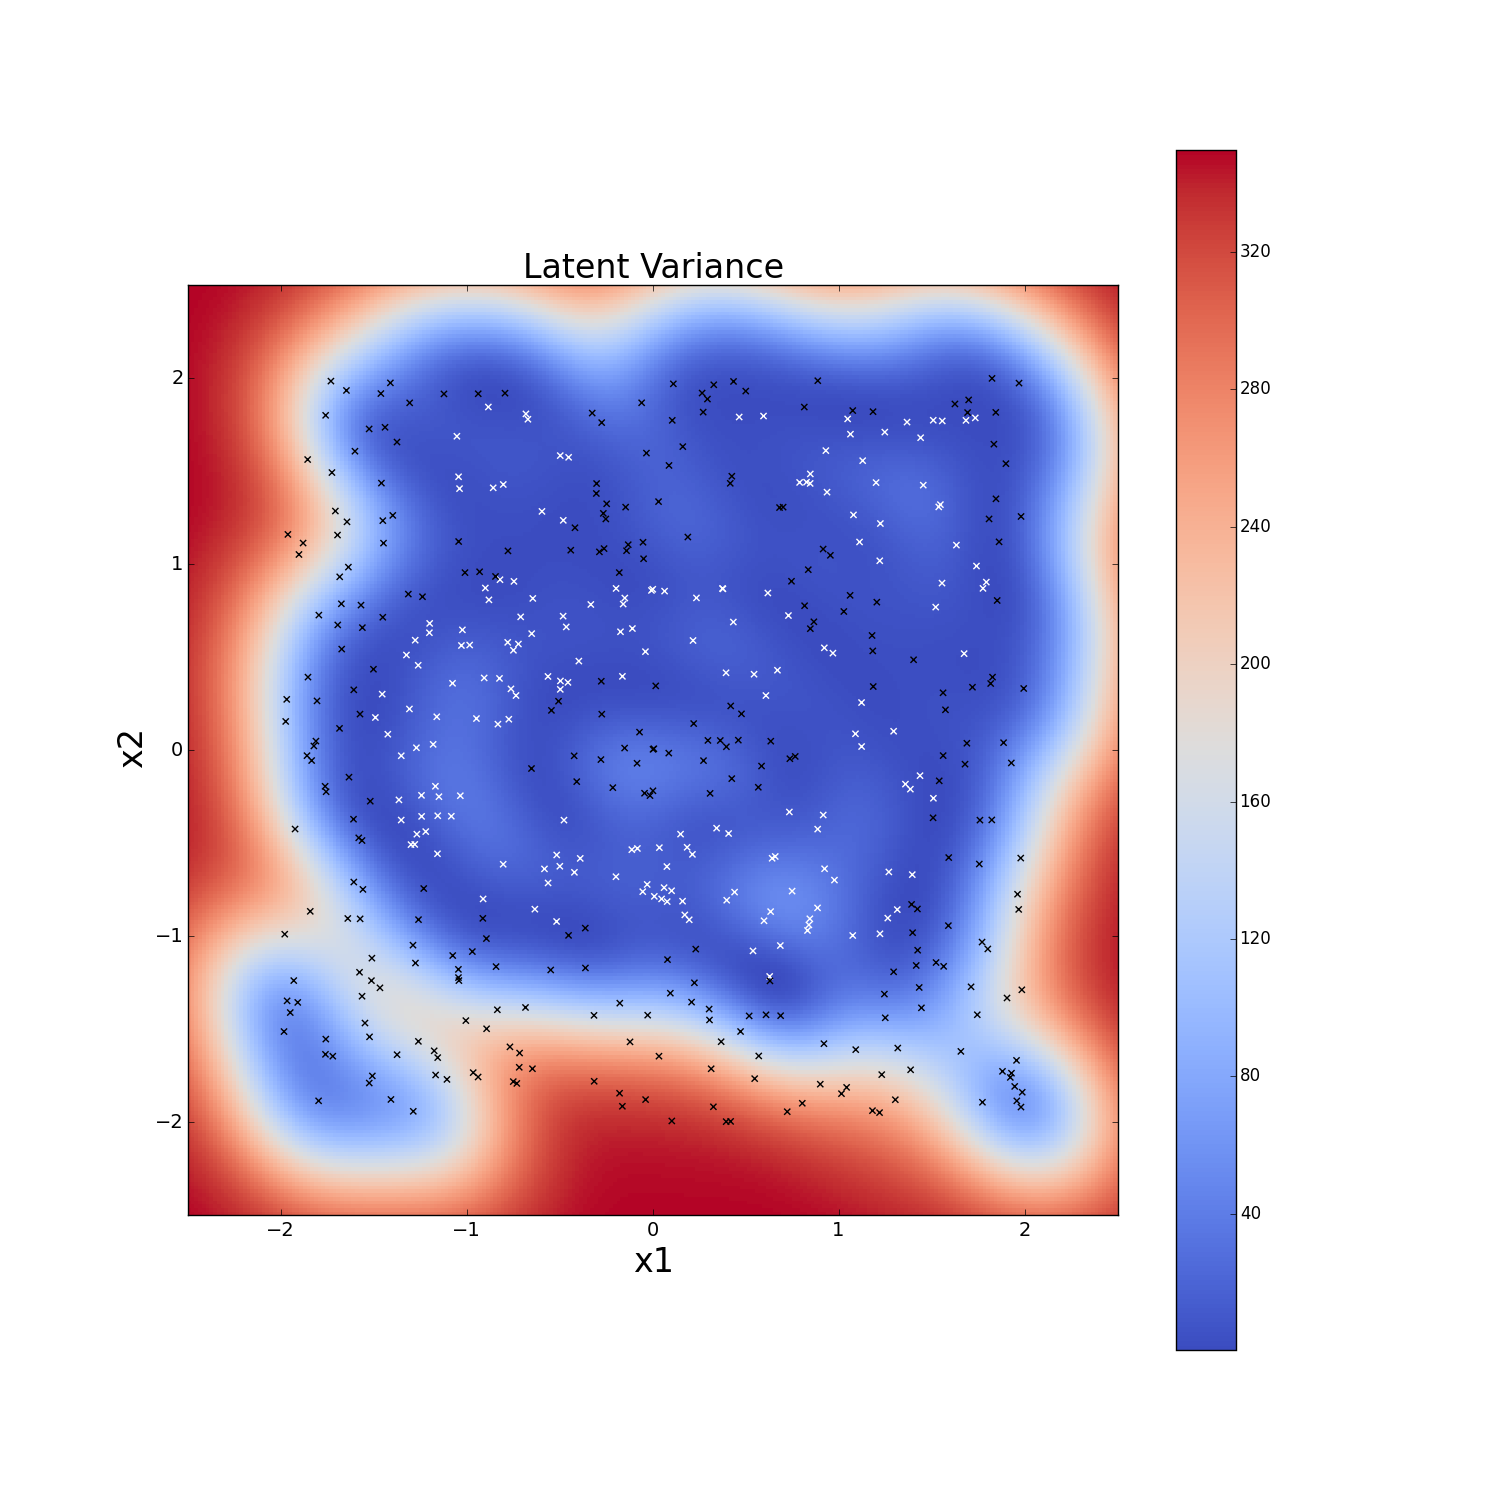
\includegraphics[width=0.48\linewidth]{Figures/scott_reef_mapping_one_colorbar/Figure4.eps}}
			  \subfigure{\label{Figure:ScottReefBathymetricFeatures:5}	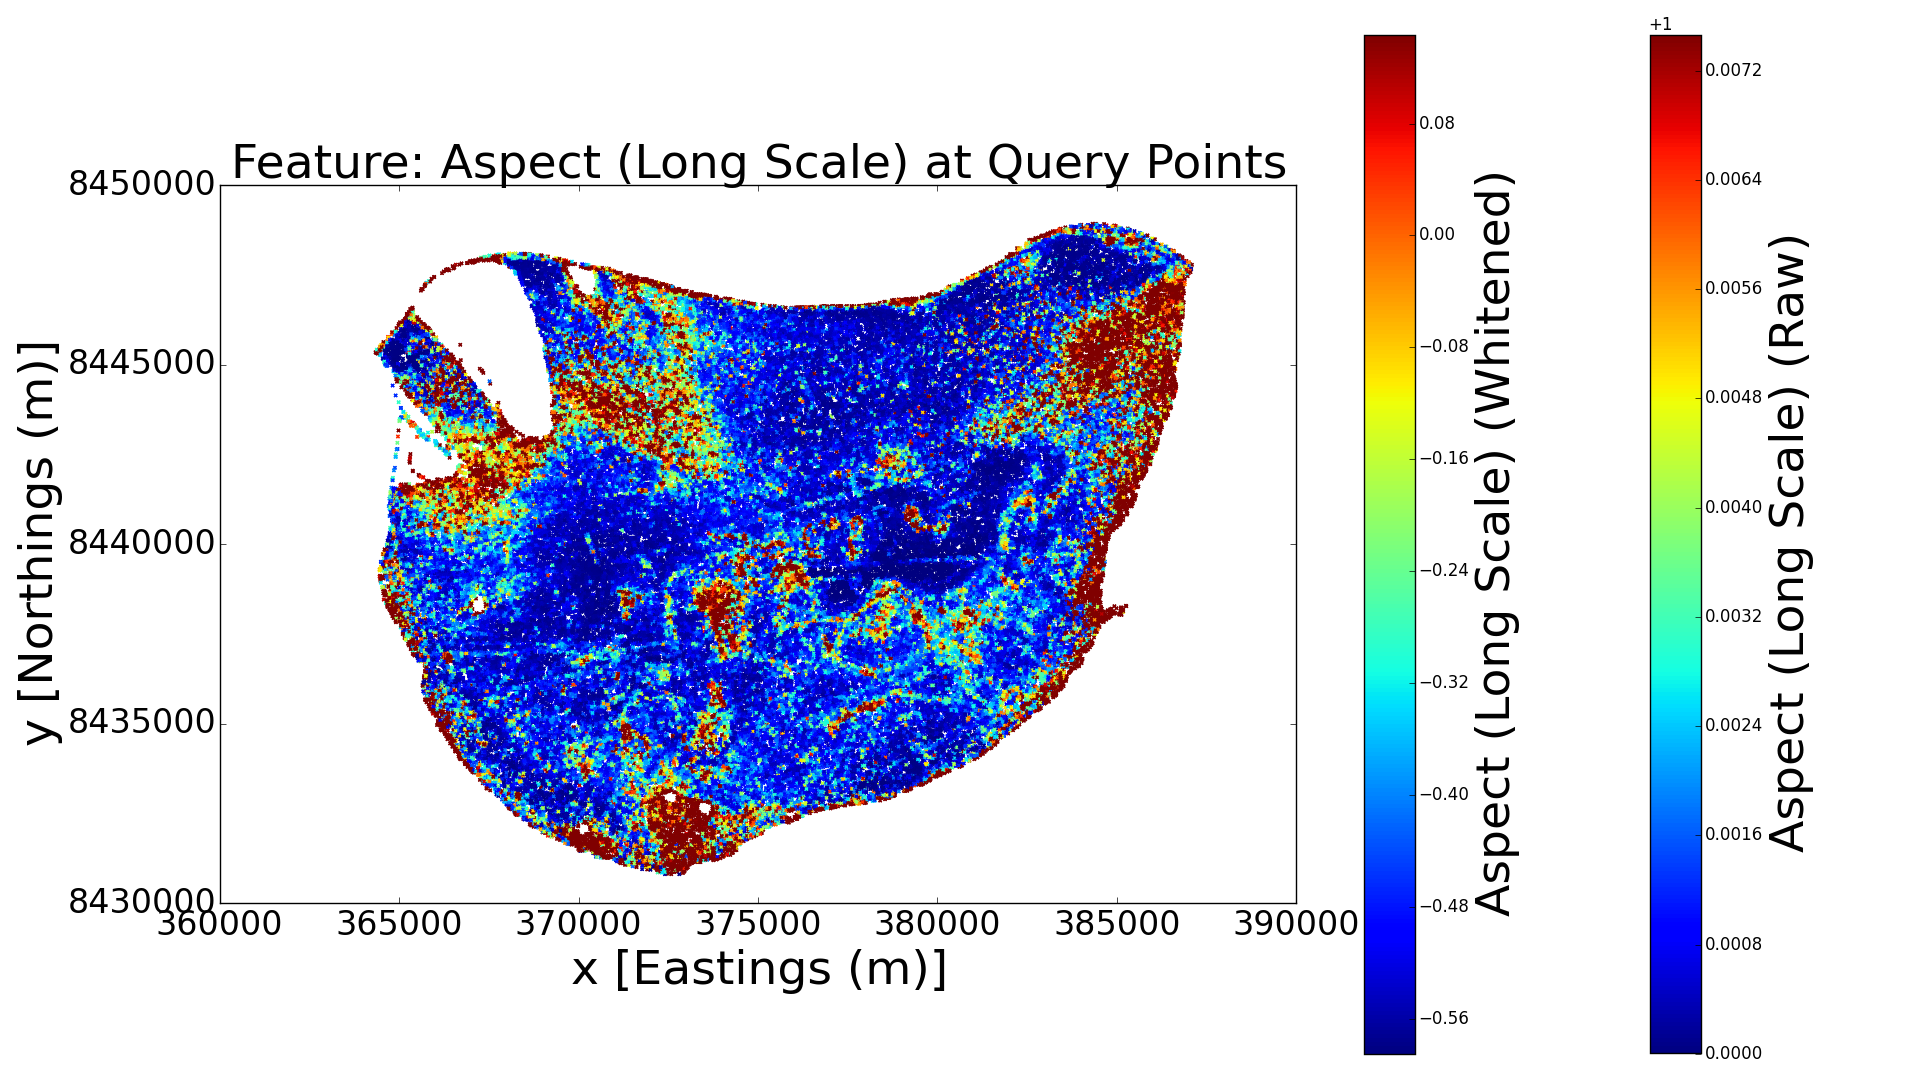
\includegraphics[width=0.48\linewidth]{Figures/scott_reef_mapping_one_colorbar/Figure5.eps}}
			  \subfigure{\label{Figure:ScottReefBathymetricFeatures:6}	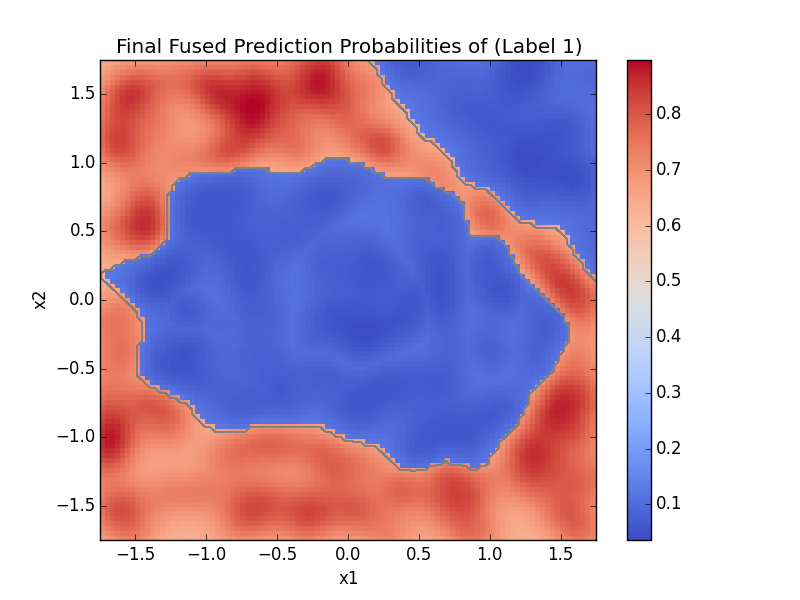
\includegraphics[width=0.48\linewidth]{Figures/scott_reef_mapping_one_colorbar/Figure6.eps}}
			\caption{Scott Reef Bathymetric Features}
			\label{Figure:ScottReefBathymetricFeatures}
			\end{figure}
			
%			\begin{figure}[!htbp]
%			\centering
%				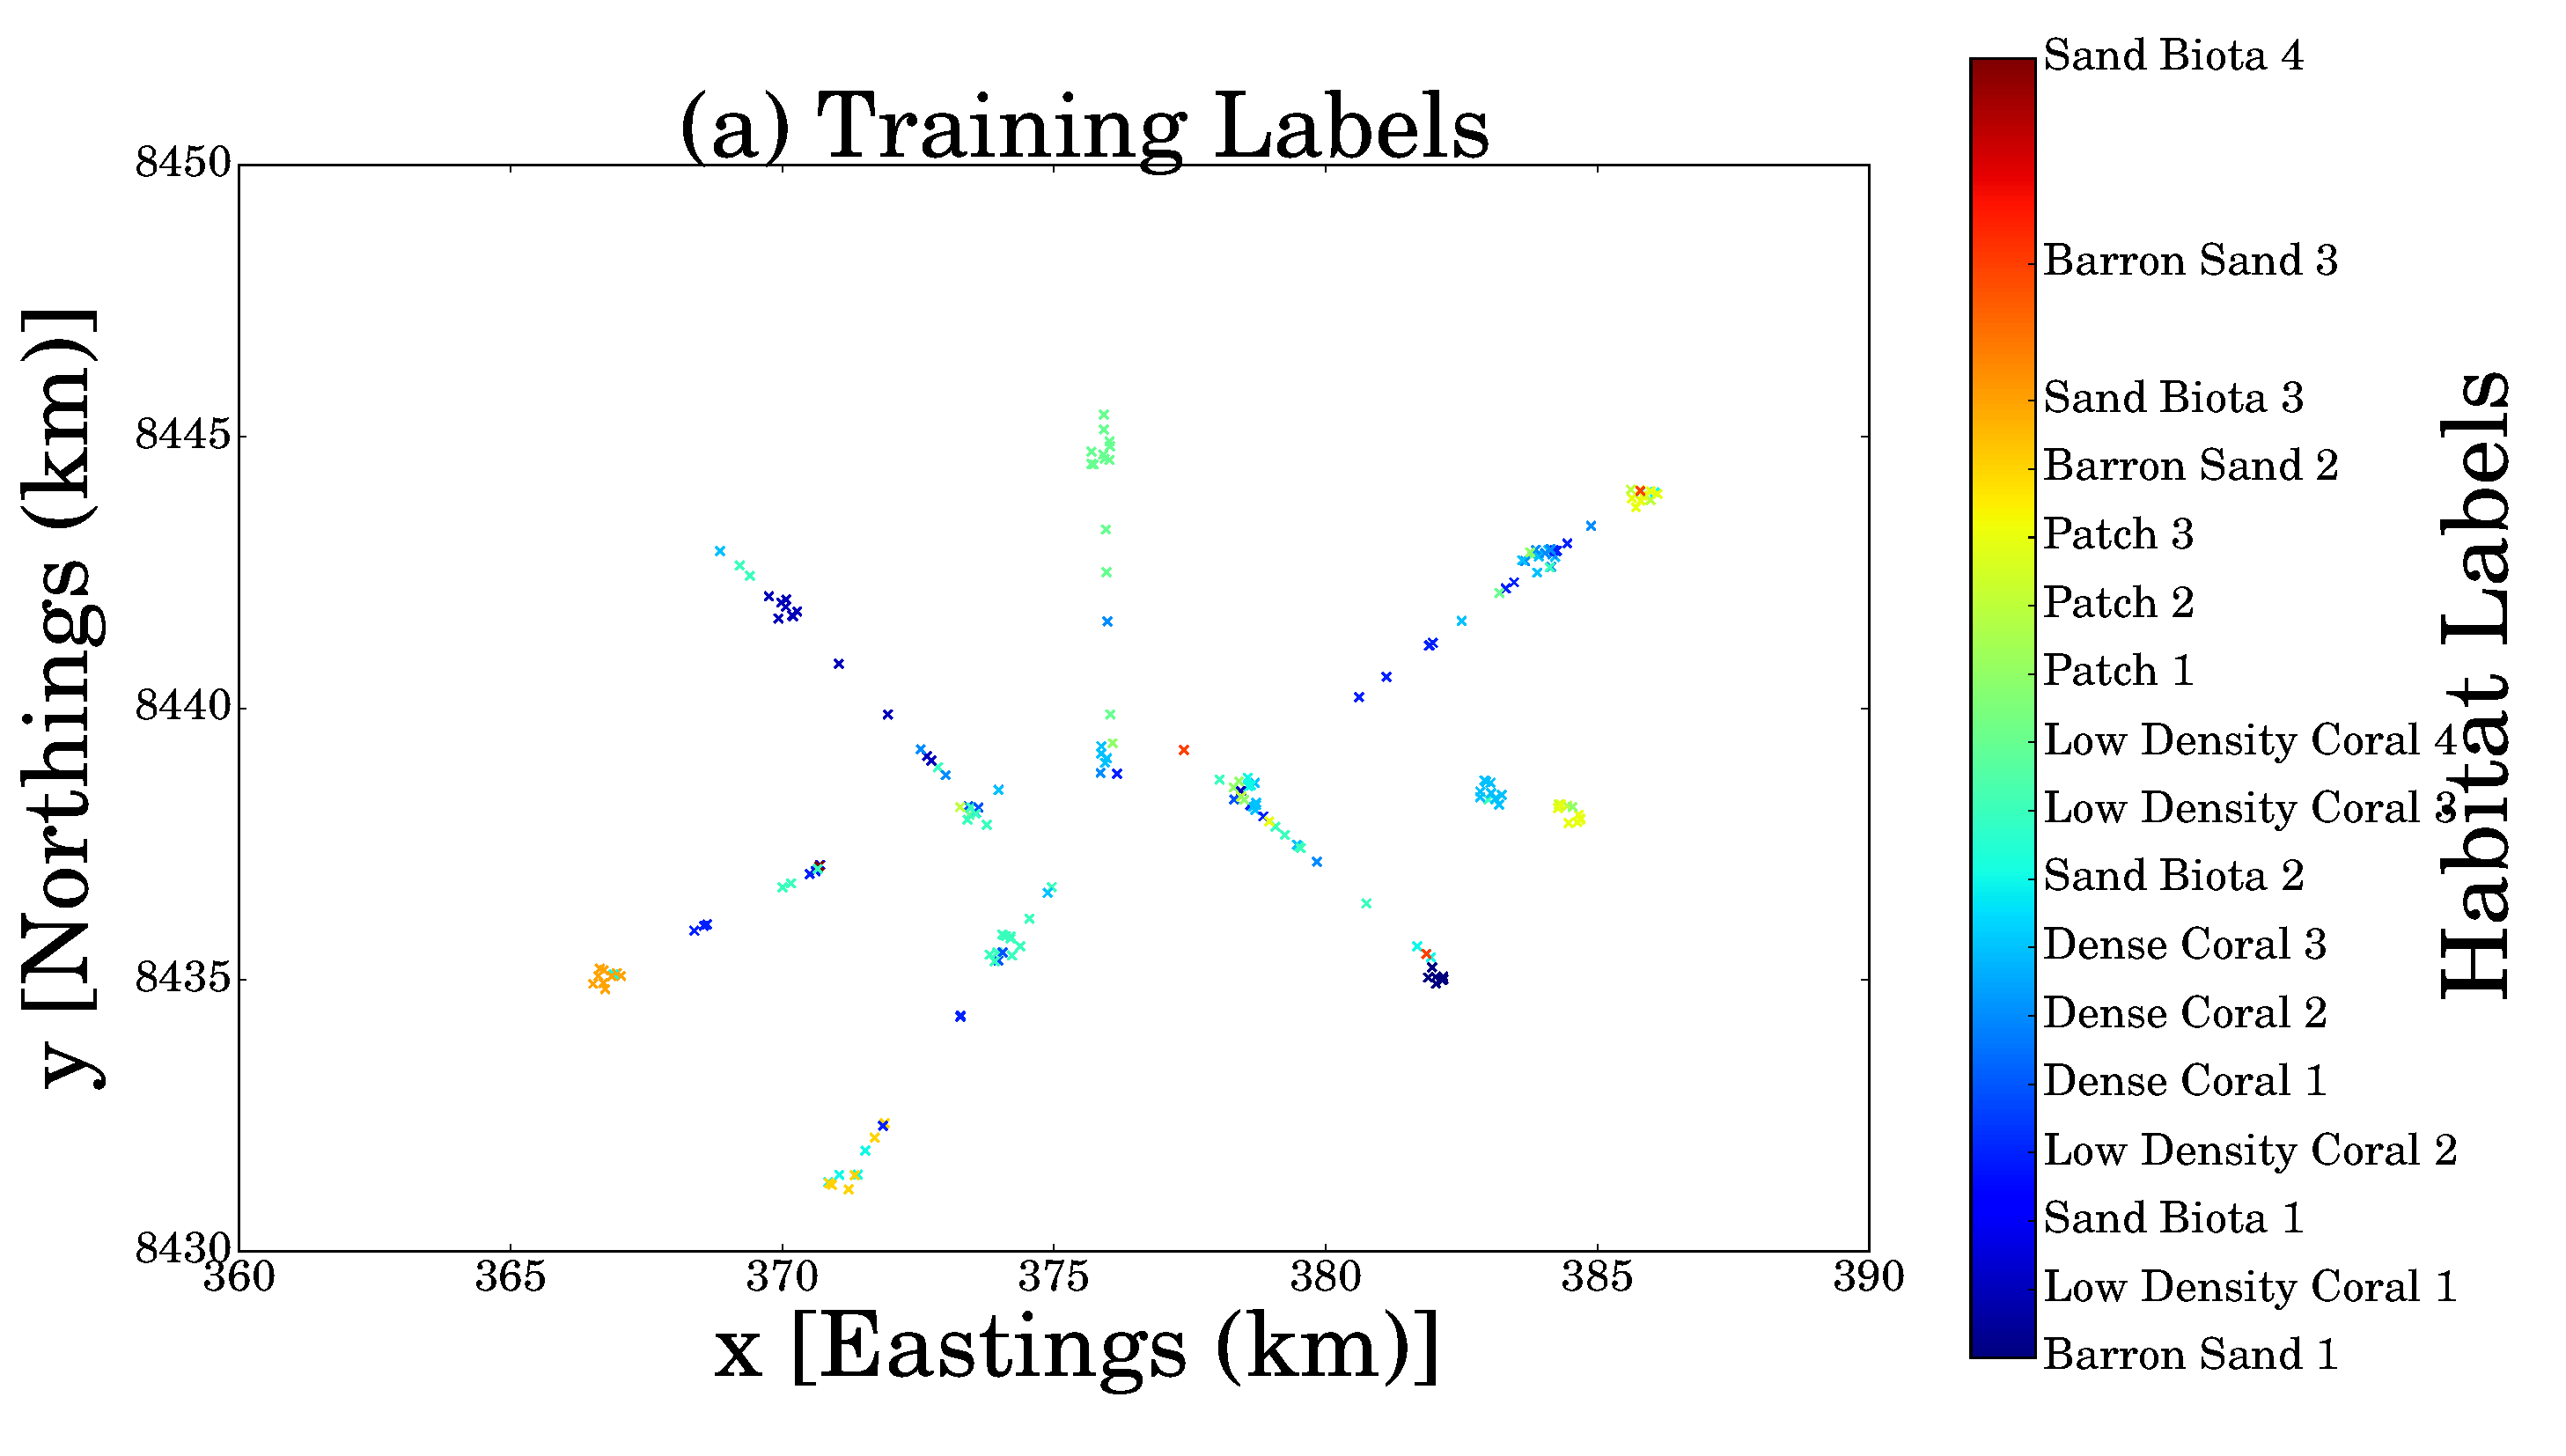
\includegraphics[width = 0.48\linewidth]{Figures/scott_reef_mapping_one_colorbar/Figure1.eps}
%				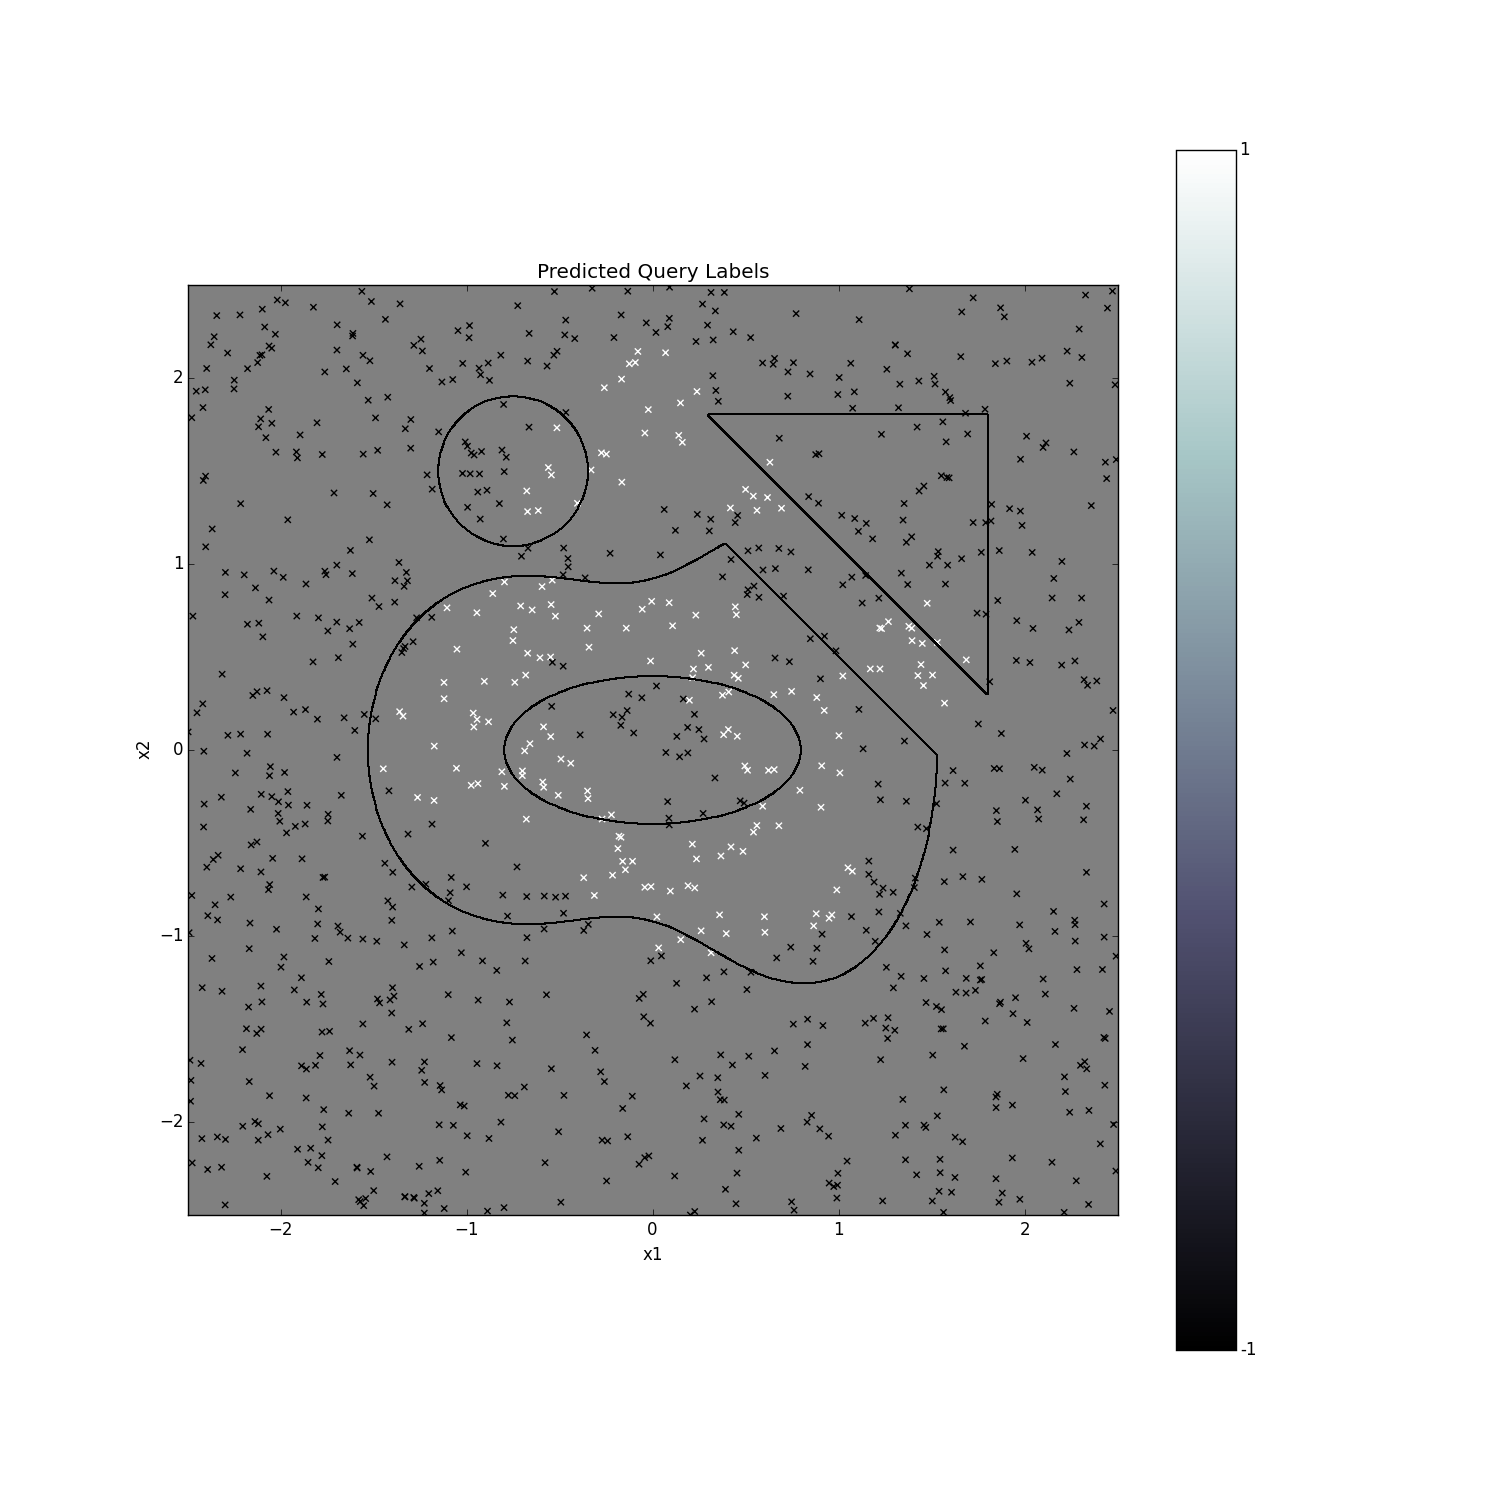
\includegraphics[width = 0.48\linewidth]{Figures/scott_reef_mapping_one_colorbar/Figure2.eps}
%				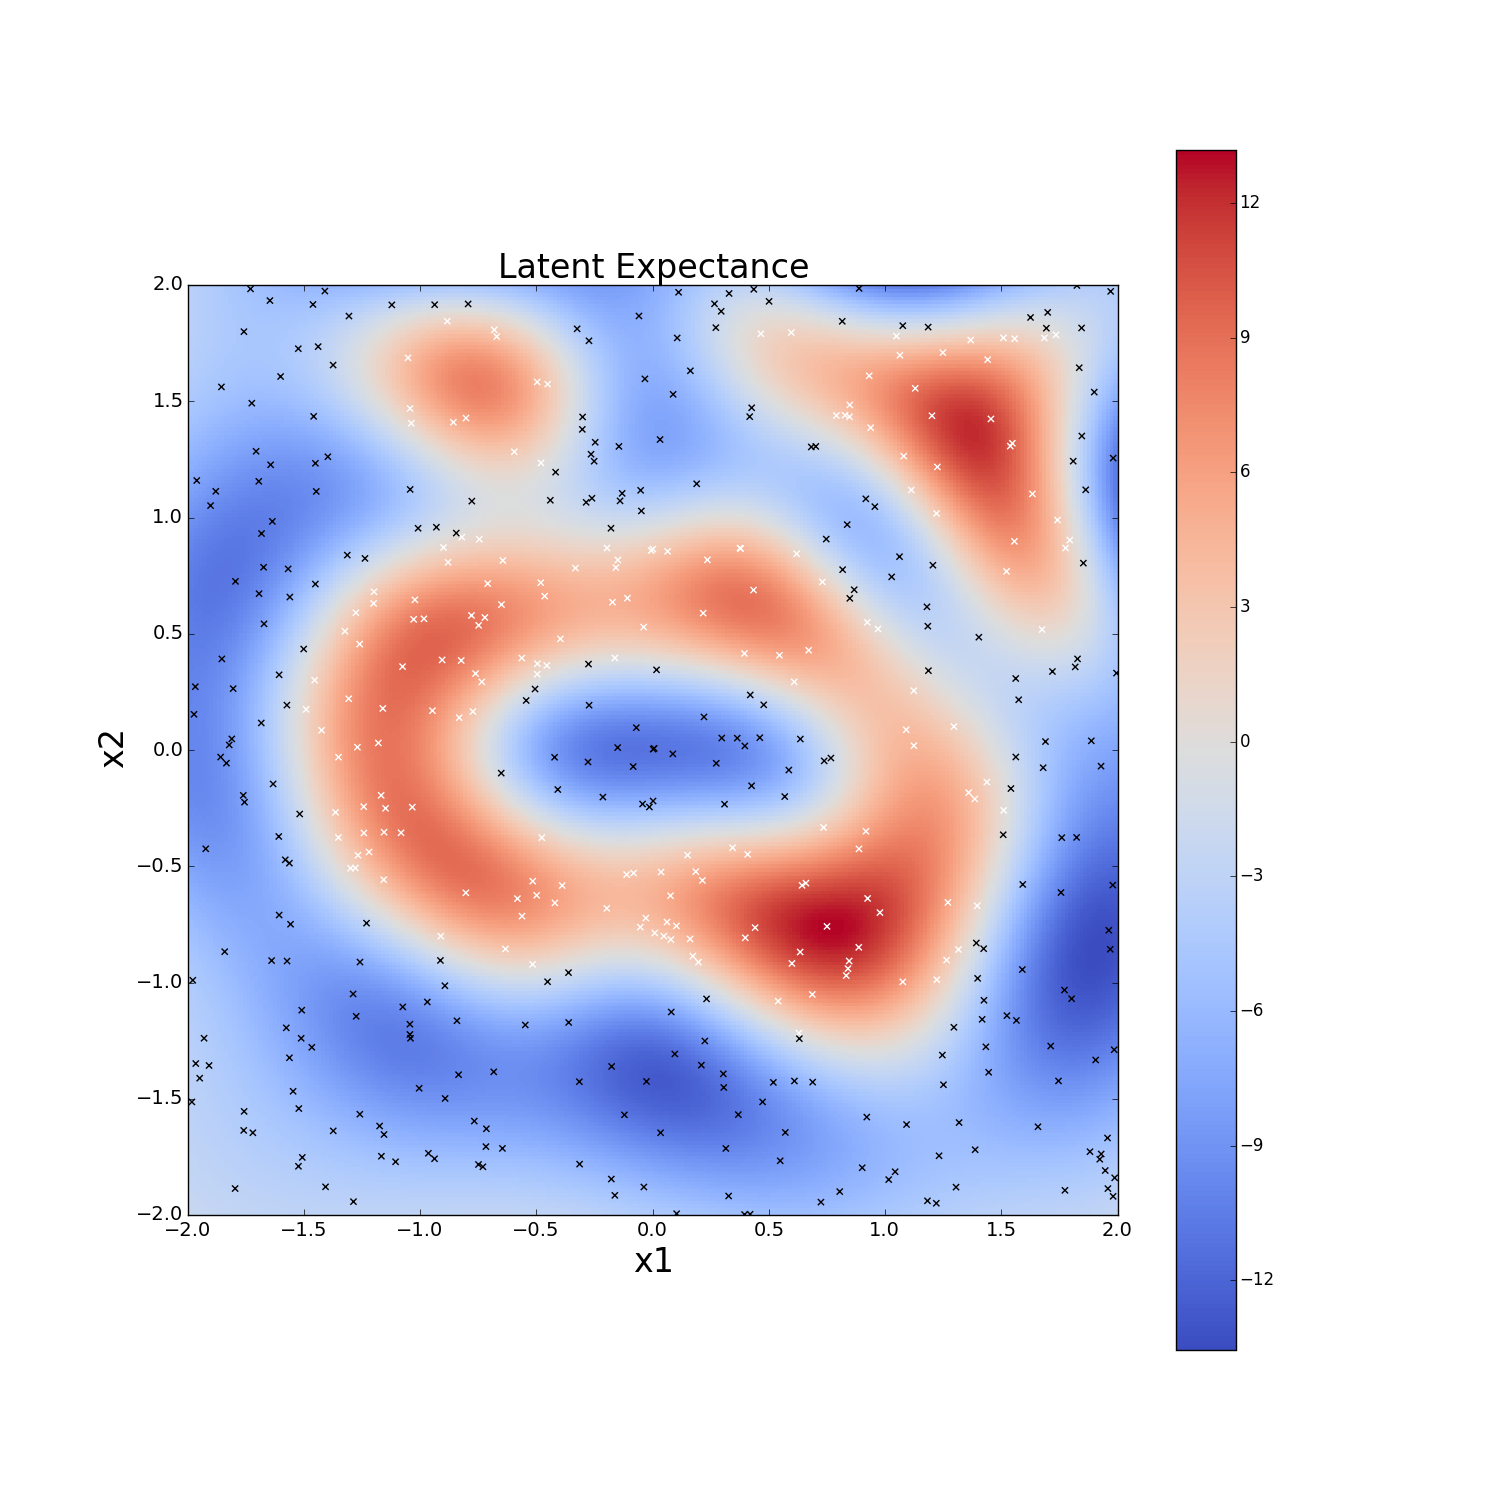
\includegraphics[width = 0.48\linewidth]{Figures/scott_reef_mapping_one_colorbar/Figure3.eps}
%				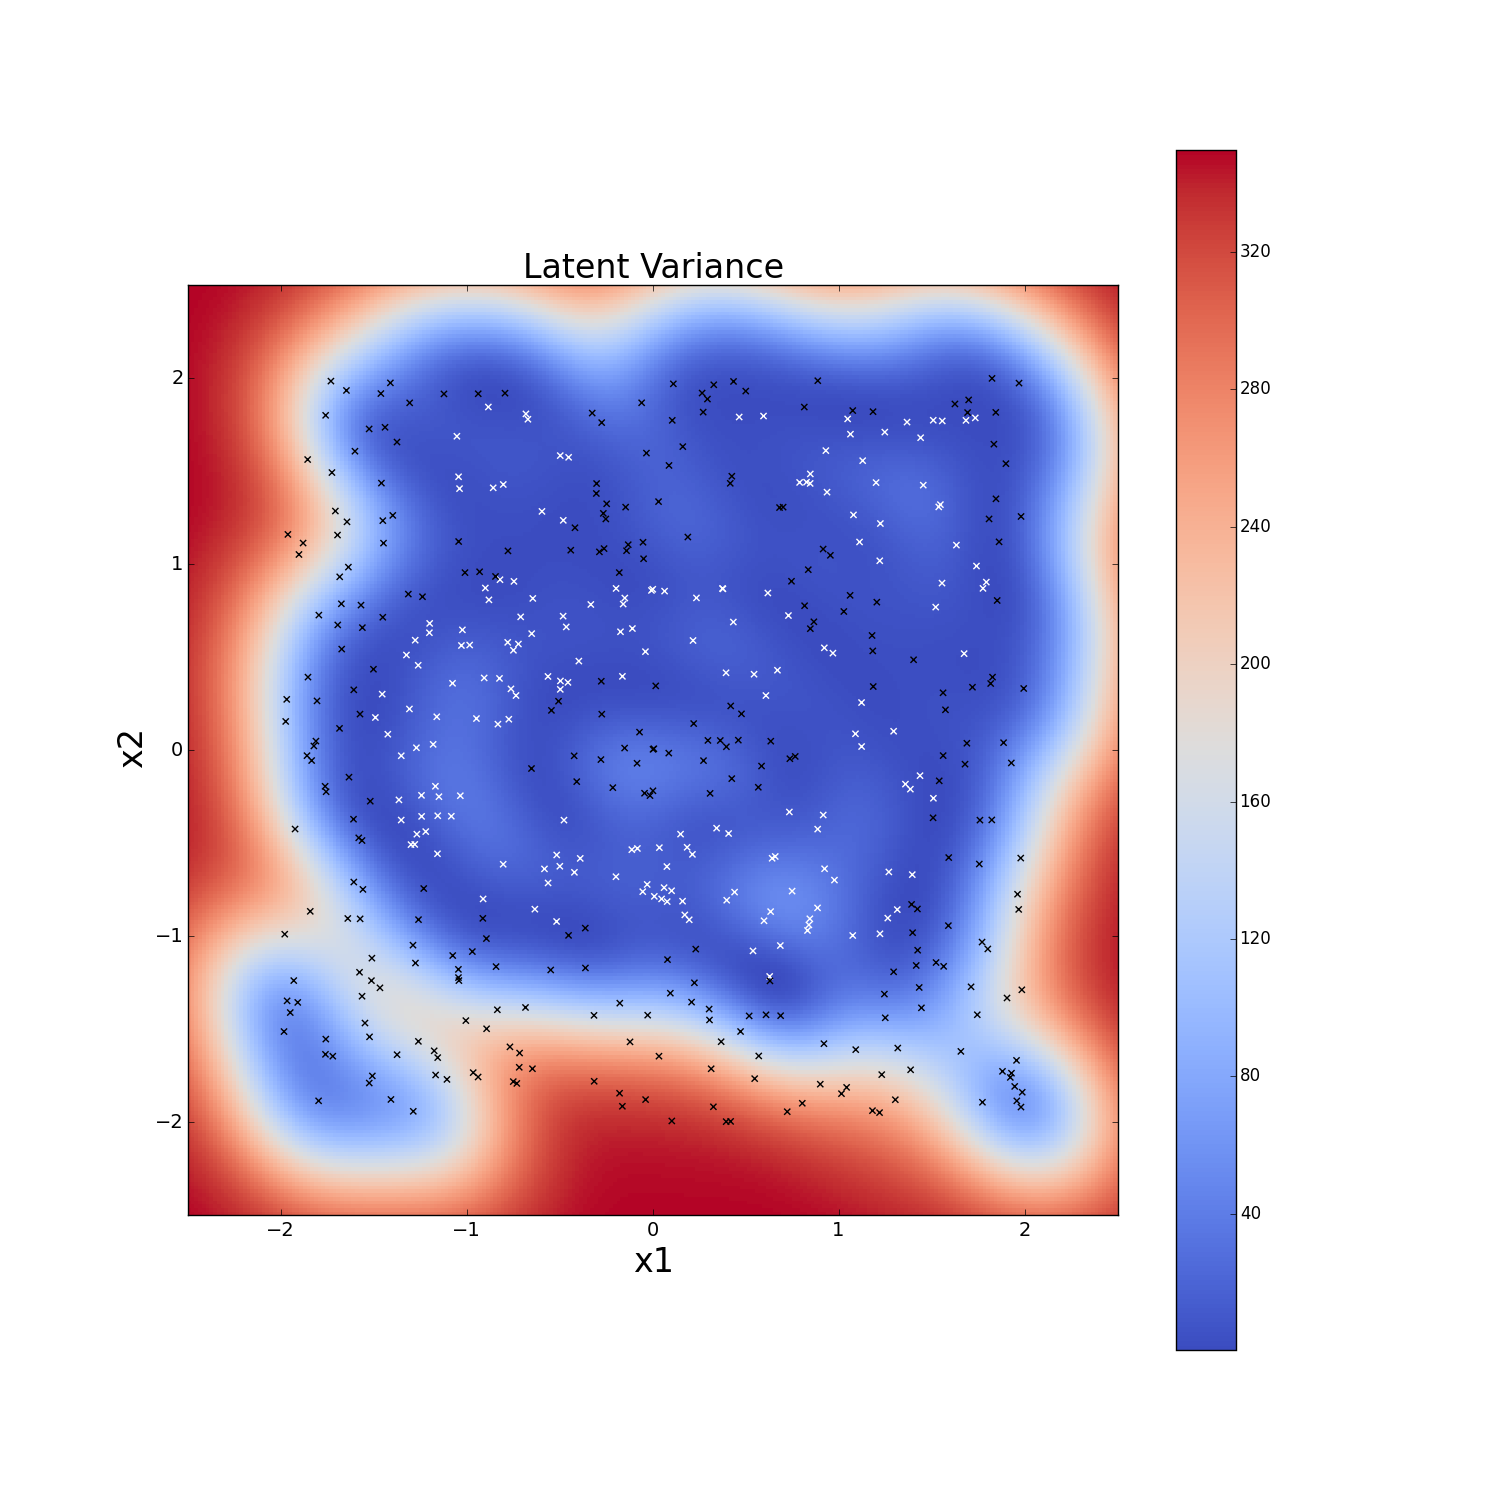
\includegraphics[width = 0.48\linewidth]{Figures/scott_reef_mapping_one_colorbar/Figure4.eps}
%				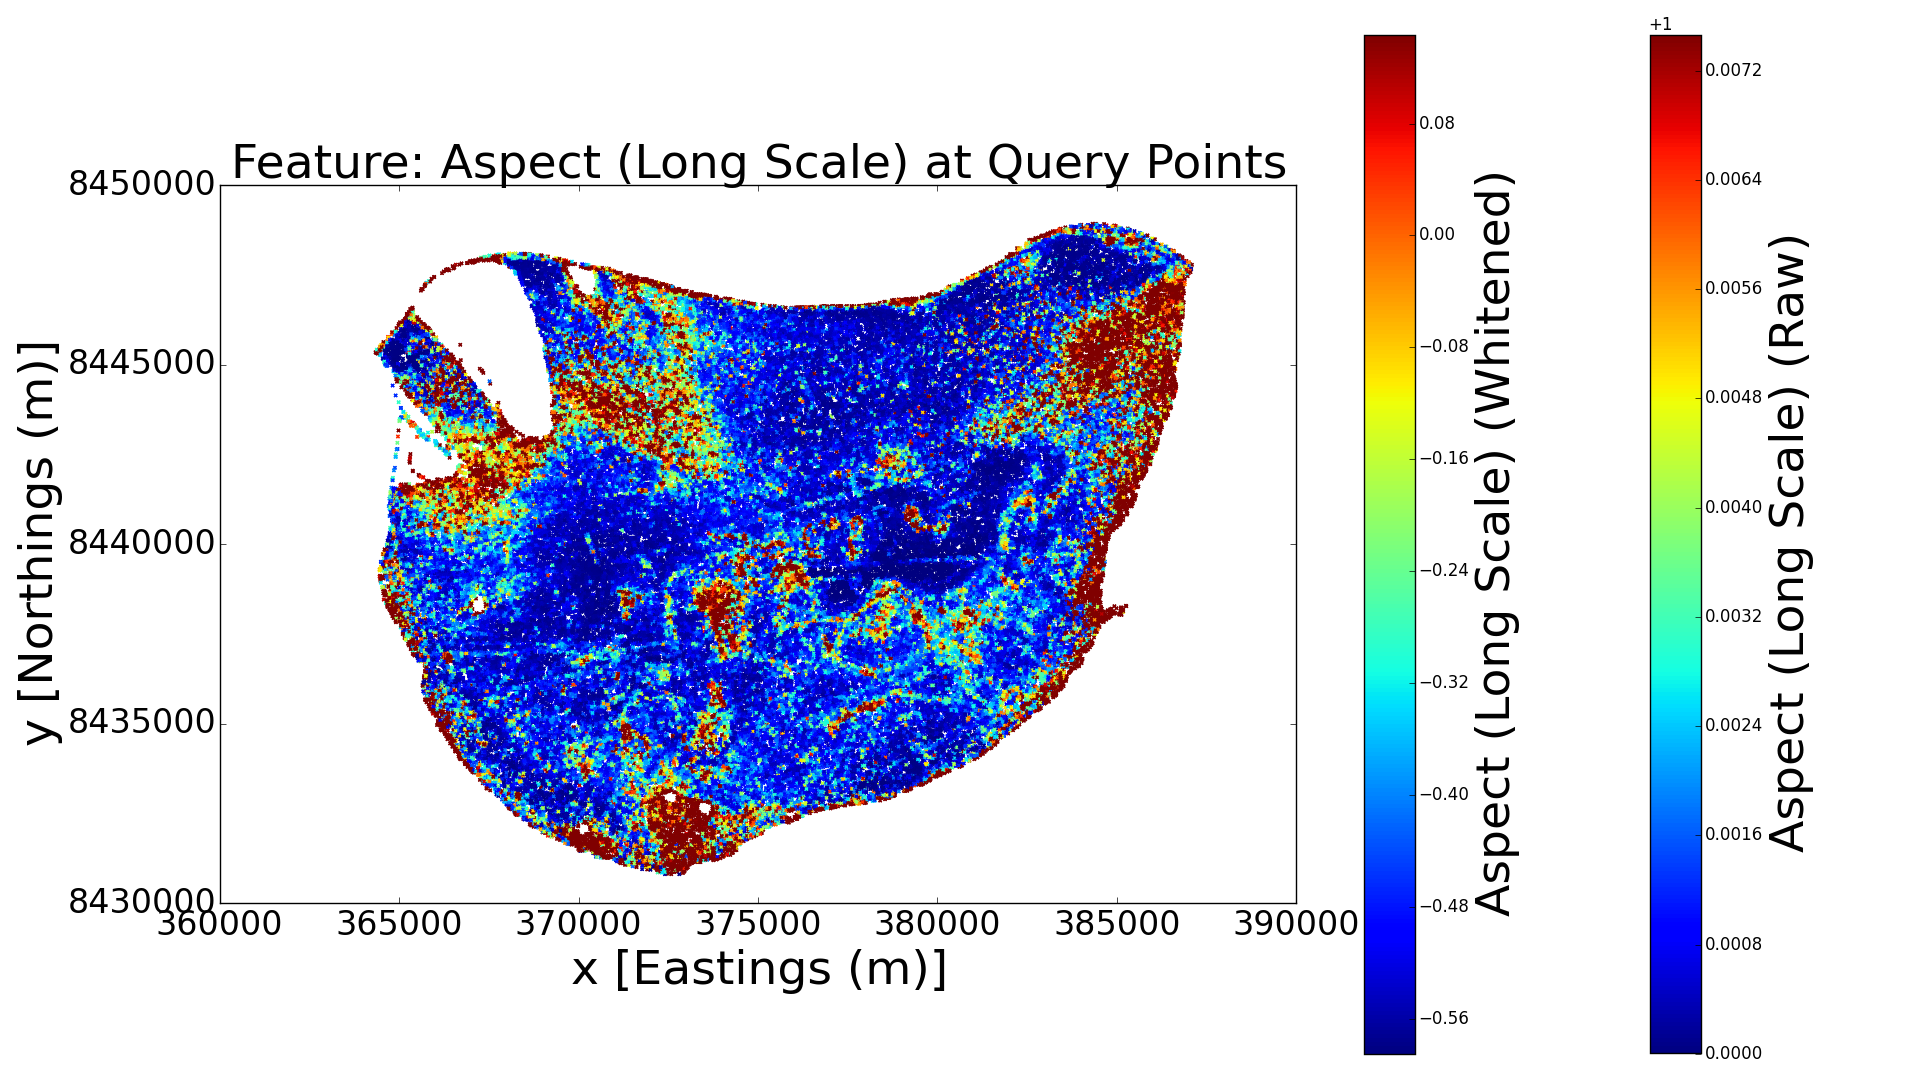
\includegraphics[width = 0.48\linewidth]{Figures/scott_reef_mapping_one_colorbar/Figure5.eps}
%				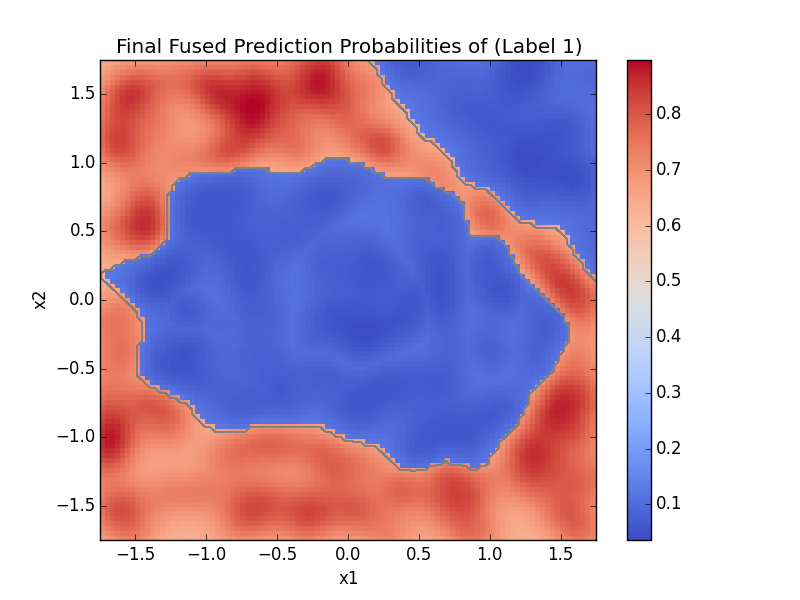
\includegraphics[width = 0.48\linewidth]{Figures/scott_reef_mapping_one_colorbar/Figure6.eps}
%			\caption{Scott Reef Bathymetric Features}
%			\label{Figure:ScottReefBathymetricFeatures}
%			\end{figure}
			
			Like the Scott Reef dataset, in most cases the bathymetric observations span the entire region of interest densely. However, while bathymetric data are usually collected rather uniformly and densely, the label data are collected from past AUV missions whose trajectory are continuous paths across the ocean floor \citep{Squidle}. Often times, these paths are approximate line segments which cover a very limited portion of the region of interest. Due to slower AUV velocity as compared to surface ships which often employ SONAR or LIDAR techniques for bathymetry mapping, the label data are also spatially denser and concentrated on the mission trajectory, while being almost non-existent elsewhere, making it a multi-modal distributed dataset. 
			
			Therefore, in order for the GP classifier to learn the relationship between the bathymetric features and habitat labels, the bathymetric data and label data must have a one-to-one correspondence. In other words, they must exist at the same locations. 
			
			Formally, let $P_{b}, P_{h} \in \mathcal{P}$ be the spatial positions at which bathymetric data and habitat label data have been observed. Let $X_{b} \in \mathcal{X}$ be the bathymetric features observed at $P_{b}$ and $\bvec{y}_{h} \in \mathcal{Y}$ be the habitat labels observed at $P_{h}$. The data matching problem is to obtain or infer $X_{h} \in \mathcal{X}$, the bathymetric features at locations $P_{h}$, from $X_{b}$.
			
			This is a standard supervised learning problem. Specifically, the aim is to learn an inference model $\zeta: P_{h} \mapsto X_{h}$ from the empirical relationship $P_{b} \mapsto X_{b}$.
			
			While it is possible to employ a separate GP regressor to perform the above inference, this adds unnecessary computational complexity. Since GPs are $O(n^{3})$ algorithms, using a layered GP approach where both stages of the benthic habitat mapping process employs GPs will increase the inference bottleneck.
			
			Instead, as there exists an abundance of bathymetric data, without much loss of accuracy it suffices to employ a nearest neighbour interpolation to obtain $X_{h}$. 
			
%			Therefore, in order to predict label data, the training data would need to be matched accurately. There are two straight forward choices at hand. The first is to estimate the bathymetric features at places where label data exists. However, at places near past mission paths, bathymetric data appears much more sparsely than label data, so that the feature extraction or regression prediction will yield very similar features across manly label data points. This reduces prediction power through a slow varying and limited feature group.
%			
%			Instead, the second choice is to estimate the label data at places where bathymetric data exists. In this setting, regions closer to past mission paths have higher volumes of label data, increasing the amount of training points. Regions further away would naturally generate more prediction uncertainty in the prediction stage.
%			
%			Hence, second method is chosen to be employed for data matching, in order to form our training set. Naturally, to predict environment labels from bathymetric features, we again need the Gaussian process classification model.
			
			\FloatBarrier
	
		\subsection{Feature Extraction}
		\label{BenthicHabitatMapping:BathymetricFeatures:FeatureExtraction}
		
			The feature extraction process assumes that the bathymetric depth data is available in grid form. That is, one can represent the available depth data $Z = \{z_{k}\}_{k \in {1, 2, ..., N}}$ as $Z = \{z_{ij}\}_{i \in {1, 2, ..., n_{i}}, \;\; j \in {1, 2, ..., n_{j}}}$ where varying $i$ and $j$ corresponds to varying data points in axis 1 and 2 respectively. Axis 1 and 2 is required to form an orthonormal frame. While axis 1 and 2 is usually aligned with the eastings-northings frame, it is generally not required for the feature extraction process.
			
			Without loss of generality, let $x$ and $y$ denote quantities corresponding to the orthogonal axes. We have that at $(x_{i}, y_{j})$ $(i \in {1, 2, ..., n_{i}}, \;\; j \in {1, 2, ..., n_{j}})$ the depth is measured as $z_{ij}$. The partial derivatives of various degrees of accuracy and scale can then be estimated through central differencing. Table \ref{Table:AspectExtraction}  shows the case for extracting aspect in the $x$-direction. Correspondingly, replacing the operations from $i$ to $j$ the aspect in the $y$-direction can also be similarly extracted.
			
			\bgroup
			\def\arraystretch{2}%  1 is the default, change whatever you need
			\begin{table}[h]
				\begin{center}
					\begin{tabular}{ c c }
						\hline
						\hline
						N & Aspect (Slope) Extraction [$x$-direction]\\
						\hline
						\hline
						3 & $^{3}_{x}a_{i, j} := \frac{- z_{i - 1, j} + z_{i + 1, j}}{2h}$ \\
						5 & $^{5}_{x}a_{i, j} := \frac{z_{i - 2, j} - 8 z_{i - 1, j} + 8 z_{i + 1, j} - z_{i + 2, j}}{12h}$ \\
						7 & $^{7}_{x}a_{i, j} := \frac{-z_{i - 3, j} + 9 z_{i - 2, j} - 45 z_{i - 1, j} + 45 z_{i + 1, j} - 9 z_{i + 2, j} + z_{i + 3, j}}{60h}$ \\
						9 & $^{9}_{x}a_{i, j} := \frac{3 z_{i - 4 j} - 32 z_{i - 3, j} + 168 z_{i - 2, j} - 672 z_{i - 1, j} + 672 z_{i + 1, j} - 168 z_{i + 2, j} + 32 z_{i + 3, j} - 3 z_{i + 4, j}}{840h}$ \\
						\hline
						\hline
					\end{tabular}
				\end{center}
		  	\caption{Aspect feature extraction using finite (central) difference approximations}
		  	\label{Table:AspectExtraction}			
		  	\end{table}	
	  		\egroup
	  		
	  		The chosen spacing employed in this thesis are $N = 3$ neighbors for short scale aspect and $N = 9$ neighbors for large scale aspect. That is, \begin{align*} \numberthis \label{Equation:AspectExtraction}
	  				{_{x}\{a_{s}\}_{i, j}} &:= {^{3}_{x}a_{i, j}} \quad && {_{y}\{a_{s}\}_{i, j}} := {^{3}_{y}a_{i, j}} \quad && {\{a_{s}\}_{i, j}} := \sqrt{{_{x}\{a_{s}\}^{2}_{i, j}} + {_{y}\{a_{s}\}^{2}_{i, j}}} \\
	  				{_{x}\{a_{l}\}_{i, j}} &:= {^{9}_{x}a_{i, j}} \quad && {_{y}\{a_{l}\}_{i, j}} := {^{9}_{y}a_{i, j}} \quad && {\{a_{l}\}_{i, j}} := \sqrt{{_{x}\{a_{l}\}^{2}_{i, j}} + {_{y}\{a_{l}\}^{2}_{i, j}}}
	  		\end{align*}
	  						  					
			Central differencing is chosen as it is more numerically accurate. The disadvantages of instability and slightly higher time complexity from dynamic cases are not present in the static feature extraction process. Nevertheless, forward differencing is to be used at the boundaries of the dataset where neighboring data is missing on one side.
						
			With two axis, the result is a 2 element gradient vector. It is possible to treat the 2 elements as separate features. However, this would make the modeling problem frame dependent which would unnecessarily complicate the modeling process. Therefore, the magnitude of this gradient is taken as the aspect feature \eqref{Equation:AspectExtraction}. 
			
			Rugosity is a measure of local height variations in the terrain. By definition, it is computed with $r = A_{r}/A_{g}$, the real surface area divided by the geometric surface area. Under bathymetry measurements that are geo-referenced through stereo imagery, rugosity can be calculated through a Delaunay triangulated surface mesh and projecting areas onto the plane of best fit using Principal Component Analysis (PCA) \citep{Friedman:Rugosity}.
							
			\FloatBarrier
				
	\section{Gaussian Process Classification}
	\label{BenthicHabitatMapping:Classification}
	
		After extracting the bathymetric features across the seafloor terrain, the next step in benthic habitat mapping is to develop a classification algorithm for habitat class inference. Gaussian process classification is of vital importance to the benthic habitat modeling process. It is used to infer the habitat type, and most importantly quantify the information reward one can gain by exploring a given area. As concluded in section \ref{Background:RelatedWork:AcquisitoinFunctions}, there has been many prior attempts in using Gaussian process classifiers for benthic habitat mapping. However, while Gaussian process classifiers are strong in inference and predictive ability, its use is complicated by its lack of analytical tractability. Approximate solutions are therefore required. Furthermore, it is non-trivial to formulate a Gaussian process based multiclass classifier, as well as ensuring a consistent predictive probability distribution from the resulting multiclass classifier. This section address those concerns and outlines the basic formulation of Gaussian process classifiers.
		
		Unlike the regression case described in section \ref{Background:GaussianProcesses:Regression}, the analytical intractability is caused by a non-Gaussian likelihood response $p(\bvec{y} | \bvec{f}, \vec{\uptheta})$, since the output labels are no longer continuous \eqref{Equation:ClassificationLogMarginalLikelihoodBayes}. Note that there is no noise parameter $\sigma$ involved, so that the hyperparameters are $\vec{\uptheta}$ in accordance to the notations introduced in section \ref{Background:GaussianProcesses:Regression}.

		\begin{equation}
			\overbrace{p(\bvec{f} | \bvec{y}, \vec{\uptheta})}^{\mathclap{\substack{\text{Non-Gaussian} \\ \text{as a result}}}} = \frac{\overbrace{p(\bvec{y} | \bvec{f}, \vec{\uptheta})}^{\text{Non-Gaussian}} \; \overbrace{p(\bvec{f} | \vec{\uptheta})}^{\text{Gaussian}}}{\underbrace{p(\bvec{y} | \vec{\uptheta})}_{\mathclap{\substack{= \int\limits_{\mathbb{R}^{n}} p(\bvec{y} | \bvec{f}, \vec{\uptheta})) p(\bvec{f} | \vec{\uptheta})) d\bvec{f} \\ \Rightarrow \; \text{Non-Gaussian due to above}}}}}
		\label{Equation:ClassificationLogMarginalLikelihoodBayes}
		\end{equation}

		The above Bayes relation \eqref{Equation:ClassificationLogMarginalLikelihoodBayes} demonstrates that the posterior probability is in general not Gaussian. In this way, approximations are necessary. Four of the most popular approximations to GP classification, in increasing accuracy and computational complexity, are Probabilistic Least Squares, Laplace Approximation, Expectation Propagation, and Variational Inference \citep{GaussianProcessForMachineLearning}. As expectation propagation and variational inference is extremely computationally heavy and thus hinder tractability performances, Laplace approximation is chosen as a reasonable balance between accuracy and implementation difficulty. A short investigation of probabilistic least squares will also be provided.
		
		The general concept behind the approximation is that the posterior $p(\bvec{f} | \bvec{y}, \vec{\uptheta})$ is approximated by another (multivariate) Gaussian distribution $q(\bvec{f} | \bvec{y}, \vec{\uptheta})$ such that the latent function is still distributed as a GP for the inference process presented in Figure \ref{Figure:GaussianProcessGraphicalModel} to remain analytically tractable.
		
		In most GP classification schemes, the latent function also has a particular interpretation - it quantifies the how strongly a particular point belongs to a given class. As a binary classification example, if the classifier is to distinguish between ``apples'' and ``oranges'', the latent function would represent the ``appleness'' of each point, with high ``appleness'' corresponding to observations likely to be ``apples'' and low ``appleness'' corresponding to observations likely to be ``oranges''. Note that only one latent function is needed in the binary case and there is no need for a latent function for ``orangeness''. Intuitively, the latent function translates to a probability through being monotonically ``squashed'' into the unit range $[0, 1]$.
		
		The outset of this section, section \ref{BenthicHabitatMapping:Classification:BinaryClassification}, begins by introducing the basic theory behind binary classification. After a summarising the basics of response functions in section \ref{BenthicHabitatMapping:Classification:ResponseFunction}, the technique of Laplace approximation and probabilistic least squares approximations are then presented respectively in sections \ref{BenthicHabitatMapping:Classification:LaplaceApproximation} and \ref{BenthicHabitatMapping:Classification:ProbabilisticLeastSquaresApproximation}. These approximations are then compared in performance in section \ref{BenthicHabitatMapping:Classification:ApproximationPerformance}. This then allows the development of multiclass classification methods, which are detailed in section \ref{BenthicHabitatMapping:Classification:MulticlassClassification}. Finally, to ensure inference consistency, two novel probability fusion techniques are presented in section \ref{BenthicHabitatMapping:Classification:ProbabilityFusion} as an alternative to simple normalisation.
		
		\subsection{Binary Classification}
		\label{BenthicHabitatMapping:Classification:BinaryClassification}
			
			The goal of binary classifiers is to distinguish between two class labels as accurate as possible. In general, all classification algorithms begins by analysing the binary classification case before extending the theory to a multiclass scenario. This is usually because binary classification are much easier to formulate, as most regression techniques can be translated to a binary classifier almost painlessly.
			
			The basic concept involved is to associate positive outputs from the regressor with one of the two labels, leaving the negative outputs associated with the other label. Note that this usually means that the regression output is constructed to be centred around zero, and that there exists symmetry between positive and negative outputs such that the technique remains the same had the labels been switched. The way the association is formulated is what defines the type of classification technique that is employed.
			
			Naturally, to protect the symmetry involved as well as to simplify the formulation, it is customary to choose 1 and -1 as the target class labels $y$, so that $y \in \{-1, 1\}$. The continuous output from a regressor is simply the latent function $f(\bvec{x}) \in \mathbb{R}$. In this way, $y = 1$ are associated with $f > 0$, while $y = -1$ are associated with $f < 0$. Note that this inference process still follows the basic structure presented in Figure \ref{Figure:GaussianProcessGraphicalModel}. The specific way the target labels $y$ are associated with the latent $f$ is usually summarised by a \textit{likelihood response} $p(y | f)$. As such, the first step towards Gaussian process classification is to choose an appropriate \textit{response function}.
			
		\subsection{Response Functions}
		\label{BenthicHabitatMapping:Classification:ResponseFunction}
		
			Before discussing the various types of GP classifiers, it is important to understand the role of \textit{response functions} in Bayesian classifiers, which serves to perform the ``squashing'' described previously.

			\begin{figure}[!htbp]
				\centering
					\includegraphics[width=0.6\textwidth]{Figures/responses.eps}
				\caption{Common likelihood responses}
				\label{Figure:LikelihoodResponses}
			\end{figure}
					
			The response function, often also called a sigmoid function, is used as the likelihood model for Bayesian classifiers. These functions must satisfy the requirement that is it monotonically non-decreasing with a domain of all real numbers $\mathbb{R}$ and a range of unit interval [0, 1]. That is, $\sigma: \mathbb{R} \mapsto [0, 1]$. As referenced above, these functions serve to ``squeeze'' the latent functions into a range where probabilistic interpretation is possible.
				
			The most widely used response functions are the logistic response \eqref{Equation:LogisticResponse} and probit \footnote{The probit function is also simply the standard normal cumulative distribution. The term \textit{probit} is used to make explicit its interpretation as a response likelihood function.} response \eqref{Equation:ProbitResponse} (figure \ref{Figure:LikelihoodResponses}). After a specific response function is chosen, the likelihood is given by \eqref{Equation:LikelihoodResponse}. Note that the likelihood $p(\bvec{y}^{\star} | \bvec{f}^{\star}, \vec{\uptheta}) = p(\bvec{y}^{\star} | \bvec{f}^{\star})$ is independent of the hyperparameters $\vec{\uptheta}$ by construction. Furthermore, each target $y^{\star}_{i}$ depends only on the corresponding latent $f^{\star}_{i}$ given all the latents $\bvec{f}^{\star}$, such that with multiple latent values $\bvec{f}^{\star}$ and corresponding targets $\bvec{y}^{\star}$ the likelihood is simply the product of the likelihoods considered separately. \begin{equation}
				\sigma(z) = \frac{1}{1 + \exp(-z)}
			\label{Equation:LogisticResponse}
			\end{equation} \begin{equation}
				\sigma(z) = \Phi(z) := \int\limits_{-\infty}^{z} \phi(x) dx =  \int\limits_{-\infty}^{z} \frac{1}{\sqrt{2 \pi}} \exp\Big(- \frac{1}{2} x^{2}\Big) dx
			\label{Equation:ProbitResponse}
			\end{equation} \begin{equation}
				p(y^{\star}_{i} | f^{\star}_{i}) = \sigma(y^{\star}_{i} f^{\star}_{i}) \implies p(\bvec{y}^{\star} | \bvec{f}^{\star}) = \prod_{i = 1}^{n} p(y^{\star}_{i} | f^{\star}_{i}) = \prod_{i = 1}^{n} \sigma(y^{\star}_{i} f^{\star}_{i})
			\label{Equation:LikelihoodResponse}
			\end{equation}				
			
			In a binary case, since $y^{\star}_{i} \in \{-1, 1\}$, it is customary to define $\pi^{\star}_{i} := p(y^{\star}_{i} = 1 | f^{\star}_{i})$ as the probability of observing label $y^{\star}_{i} = 1$ given the latent value $f^{\star}_{i}$. Note that $\pi^{\star}_{i}$ is still a random variable since $f_{i}$ is a latent random variable. In this way, the probability of observing label $y_{i} = -1$ given the latent value $f^{\star}_{i}$ is simply $1 - \pi^{\star}_{i}$. As such, at the query locations $X^{\star}$, the random vector $\vec{\uppi}^{\star} := \{\pi^{\star}_{i}\}_{i \in I_{n^{\star}}}$ defines the distribution at the query locations completely.
			
			By \eqref{Equation:LikelihoodResponse}, this means that $\pi^{\star}_{i} = \sigma(f^{\star}_{i})$, which provides a simple relationship between the latent function and the predictive probability, and achieves the ``squashing'' effect mentioned previously. The vector form of this relationship can be written as $\vec{\uppi}^{\star} = \vec{\upsigma}(\bvec{f}^{\star}) := \{\sigma(f^{\star}_{i})\}_{i \in I_{n^{\star}}}$. Again, if $\bvec{f}^{\star}$ is random, then so is $\vec{\uppi}^{\star}$.
			
			In order to perform prediction, the predictive probabilities $\vec{\uppi}^{\star}$ must be known. However, given the above likelihood response formulation, since $\vec{\uppi}^{\star}$ is random, further inference must be obtained by taking the \textit{expected prediction probabilities} $\bar{\vec{\uppi}}^{\star} := \mathbb{E}[\vec{\uppi}^{\star}] = \mathbb{E}[\vec{\upsigma}(\bvec{f}^{\star})]$ for inference \eqref{Equation:PriorExpectedPredictionProbabilities}. Of course, since $f$ is formulated as a GP, the distribution of $\bvec{f}^{\star}$, $p(\bvec{f}^{\star})$, is requires the optimally learned hyperparameters $\vec{\uptheta}$. This fact is notated explicitly in \eqref{Equation:PriorExpectedPredictionProbabilities}.
			
			\begin{equation}
				\bar{\vec{\uppi}}^{\star} |_{\vec{\uptheta}} := \mathbb{E}_{\vec{\uptheta}}[\vec{\uppi}^{\star}] = \mathbb{E}_{\vec{\uptheta}}[\vec{\upsigma}(\bvec{f}^{\star})] = \int_{\mathbb{R}^{n^{\star}}} \vec{\upsigma}(\bvec{f}^{\star}) p(\bvec{f}^{\star} | \vec{\uptheta}) d \bvec{f}^{\star}
			\label{Equation:PriorExpectedPredictionProbabilities}
			\end{equation}	
			
			 Note that without any observations $\bvec{y}$ the prior distribution $p(\bvec{f}^{\star} | \vec{\uptheta})$ will be centred around zero mean. Since the response function $\vec{\upsigma}$ maps zero latents to a probability of 0.5, the expected predictive probabilities also become $\bar{\pi}^{\star}_{i} |_{\vec{\uptheta}} = 0.5$ for $i \in I_{n^{\star}}$. This reflects that before any observations, the targets at the query points have an equal chance of being -1 or 1, which indeed makes sense.
			 
			 With observations $\bvec{y}$, the expected predictive probabilities is computed by the conditionally expectation on $\bvec{y}$ using the posterior distribution $p(\bvec{f}^{\star} | \bvec{y}, \vec{\uptheta})$ \eqref{Equation:PosteriorExpectedPredictionProbabilities}.
	
			\begin{equation}
				\bar{\vec{\uppi}}^{\star} |_{\bvec{y}, \vec{\uptheta}} := \mathbb{E}_{\vec{\uptheta}}[\vec{\uppi}^{\star} | \bvec{y}] = \mathbb{E}_{\vec{\uptheta}}[\vec{\upsigma}(\bvec{f}^{\star}) | \bvec{y}] = \int_{\mathbb{R}^{n^{\star}}} \vec{\upsigma}(\bvec{f}^{\star}) p(\bvec{f}^{\star} | \bvec{y}, \vec{\uptheta}) d \bvec{f}^{\star}
			\label{Equation:PosteriorExpectedPredictionProbabilities}
			\end{equation}	
			
			Before introducing the approximation techniques, it is worthwhile to first observe the properties of the integral \eqref{Equation:PosteriorExpectedPredictionProbabilities}. Firstly, the integral can also be written in scalar form for each query point $i \in I_{n^{\star}}$ separately \eqref{Equation:PosteriorExpectedPredictionProbabilitiesScalar}.

			\begin{equation}
				 \bar{\pi}^{\star}_{i} |_{\bvec{y}, \vec{\uptheta}} = \mathbb{E}_{\vec{\uptheta}}[\pi^{\star}_{i} | \bvec{y}] = \mathbb{E}_{\vec{\uptheta}}[\sigma(f^{\star}_{i}) | \bvec{y}] = \int_{\mathbb{R}} \sigma(f^{\star}_{i}) p(f^{\star}_{i} | \bvec{y}, \vec{\uptheta}) d f^{\star}_{i} \qquad \forall i \in I_{n^{\star}}
			\label{Equation:PosteriorExpectedPredictionProbabilitiesScalar}
			\end{equation}		
						
			For a general likelihood response $\sigma(z)$, the integral \eqref{Equation:PosteriorExpectedPredictionProbabilitiesScalar} must be computed numerically through a techniques such as \textit{quadratures}. However, if $p(f^{\star}_{i} | \bvec{y}, \vec{\uptheta})$ is a Gaussian density, and a probit response is chosen for the likelihood \eqref{Equation:ProbitResponse}, then there exists an analytical solution to the integral \eqref{Equation:PosteriorExpectedPredictionProbabilitiesScalar} and hence \eqref{Equation:PosteriorExpectedPredictionProbabilities} through vectorising, as given by \eqref{Equation:ProbitAnalyticalIntegral} \citep{GaussianProcessForMachineLearning}. This means that under an appropriate approximation technique, the probit response allows \textit{analytically tractable inference} to be performed. As such, there is significant computational advantage of choosing the probit response. Choosing the probit response also exhibits further advantages for linearisation discussed later in section \ref{InformativeSeafloorExploration:LMDE}.
			
			\begin{equation}
				 \bar{\pi}^{\star}_{i} |_{\bvec{y}, \vec{\uptheta}} = \int_{\mathbb{R}} \overbrace{\Phi(f^{\star}_{i})}^{\mathclap{\substack{\text{Probit} \\ \text{Response}}}} \overbrace{p(f^{\star}_{i} | \bvec{y}, \vec{\uptheta})}^{\text{If Gaussian}} d f^{\star}_{i} \stackrel{\mathclap{\substack{\text{Analytical} \\ \text{Solution} \\ \quad }}}{=} \Phi\Bigg(\frac{\mathbb{E}_{\vec{\uptheta}}[f^{\star}_{i} | \bvec{y}]}{\sqrt{1 + \mathbb{V}_{\vec{\uptheta}}[f^{\star}_{i} | \bvec{y}]}}\Bigg) \qquad \forall i \in I_{n^{\star}}
			\label{Equation:ProbitAnalyticalIntegral}
			\end{equation}
			
		\subsection{Laplace Approximation}
		\label{BenthicHabitatMapping:Classification:LaplaceApproximation}
		
			After choosing a response function $\sigma(z)$, the expected predictive probabilities can be computed from the posterior distribution $p(\bvec{f}^{\star} | \bvec{y}, \vec{\uptheta})$ using \eqref{Equation:PosteriorExpectedPredictionProbabilities}. The heart of all GP classifier approximation techniques then lies in approximating the posterior $p(\bvec{f}^{\star} | \bvec{y}, \vec{\uptheta})$ as a multivariate Gaussian density.
			
			Unfinished
			
		\subsection{Probabilistic Least Squares Approximation}
		\label{BenthicHabitatMapping:Classification:ProbabilisticLeastSquaresApproximation}
		
			The main difference is just the training stage!
			
			Unfinished
		\subsection{Approximation Properties \& Performance}
		\label{BenthicHabitatMapping:Classification:ApproximationPerformance}
		
			Compare probability outputs, classification outputs, entropy outputs, etc
		
			Unfinished
			
		\subsection{Multiclass Classification}
		\label{BenthicHabitatMapping:Classification:MulticlassClassification}
		
			Contrary to binary classification, multiclass classification investigates the case where there are more than two labels for target outputs to be classified into so that $n_{C} > 2$. In this case, the class labels are formulated to be in the range $y \in I_{n_{C}} = \{1, 2, \dots, n_{C}\}$ for convenience. However, not that this is not strictly necessary. Any set of labels $\mathcal{Y}$ is equivalent as long as $\Vert \mathcal{Y} \Vert = n_{C}$ such that $n_{C}$ distinct numbers are used. In other words, there must exist a one-to-one correspondence between the set of label $\mathcal{Y}$ and $I_{n_{C}}$.
			
			The previous sections established two of many approximation techniques for binary classification. While there exists a multiclass version for classification under Laplace approximation, the method requires multiple inversion stages \textit{per iteration} in the training and inference stage, and most importantly a Monte Carlo estimation stage in the inference stage. This introduces many inners loops in both the training and inference stage. As matrix inversions are $O(n^{3})$ algorithms, it is not desirable to repeat them multiple times in \textit{each iteration}, which would make the training stage significantly slower. Furthermore, the inference stage is bottlenecked by the Monte Carlo estimation loops, which introduces an accuracy-complexity trade-off that is not desirable in a big data problem such as informative seafloor exploration. Moreover, the multiclass formulation is specific to only Laplace approximation, which limits its application.
			
			As such, this thesis investigates other general methods for multiclass classification. The methods investigated are \textit{One versus All} (OVA) and \textit{All versus All} (AVA) classification.
	
			\subsubsection{One Versus All Classification}
			\label{BenthicHabitatMapping:Classification:MulticlassClassification:OVA}
						
				The OVA approach performs classification by introducing $n_{C}$ \textit{independent} classification problems, each classifying a particular label against all other labels. Each binary classifier is identified with a class label $c$, where it attempts to distinguish targets with labels $c$ against targets with any other label $c' \in I_{n^{C}} \backslash c$. Each of these problems are thus a binary classification problem for which solution methods are as demonstrated previously.
				
				The approach begins by translating the training observations from a multiclass target vector $\bvec{y} \in \{1, 2, \dots, n_{C}\}^{n}$ into $n_{C}$ binary target vectors $\bvec{y}^{c} \in \{-1, 1\}^{n}$ for $c \in \{1, 2, \dots, n_{C}\}$ \eqref{Equation:TargetTranslationOVA}.
				
				\begin{equation}
					\bvec{y}^{c} = \{\mathds{1}_{\{y_{i} = c\}} - \mathds{1}_{\{y_{i} \neq c\}}\}_{i \in I_{n}}
				\label{Equation:TargetTranslationOVA}
				\end{equation}				
				
				That is, $\bvec{y}^{c}$ is a vector of the same length as $\bvec{y}$, with its components equal to $1$ where the corresponding components of $\bvec{y}$ is equal to $c$. All other components are equal to $-1$. Here, $\mathds{1}_{A}$ is the standard notation for the indicator function, which is $1$ when $A$ is true and $0$ otherwise.
				
				As such, the binary classifier between class $c$ and all other labels is trained with the training data $(X, \bvec{y}^{c})$, and is trained independently from the other binary classifiers. Each binary classifier thus has its own set of optimal hyperparameters $\vec{\uptheta}^{c}$, and performs inference and prediction separately. This outputs a single axis list of expected predictive probabilities \eqref{Equation:ProbabilityListOVA} at all query points $X^{\star}$. Note that the query star $^{\star}$ is moved to the left to avoid cluttered notation.
				
				\begin{equation}
					\begin{Bmatrix*}
						{^{\star}}\bar{\vec{\uppi}}^{1} |_{\bvec{y}^{1}, \vec{\uptheta}^{1}} & {^{\star}}\bar{\vec{\uppi}}^{2} |_{\bvec{y}^{2}, \vec{\uptheta}^{2}} & \dots & {^{\star}}\bar{\vec{\uppi}}^{n_{C}} |_{\bvec{y}^{n_{C}}, \vec{\uptheta}^{n_{C}}}
					\end{Bmatrix*} 
				\label{Equation:ProbabilityListOVA}
				\end{equation}
				
				Once the predictive probabilities from each binary GP classifiers are obtained, a consistent framework is required for fusing the separate prediction probabilities into a coherent prediction probability. This is necessary as the binary classifiers are independently learned and performs prediction independently, and thus may not necessarily provide coherent results. In fact, simply stacking the prediction probabilities together yields a ``probability'' distribution that does not sum up to 1 \eqref{Equation:ProbabilityInconsistencyOVA}. This is the focus of section \ref{BenthicHabitatMapping:Classification:ProbabilityFusion}.

				\begin{equation}
					\sum_{c}^{n_{C}} {^{\star}}\bar{\pi}^{c}_{i} |_{\bvec{y}^{c}, \vec{\uptheta}^{c}} \stackrel{\mathclap{\substack{\text{in} \\ \text{general} \\ \quad }}}{\neq} 1 \qquad \forall i \in I_{n^{\star}}
				\label{Equation:ProbabilityInconsistencyOVA}
				\end{equation}
				
			\subsubsection{All Versus All Classification}
			\label{BenthicHabitatMapping:Classification:MulticlassClassification:AVA}
			
				The AVA approach operates in a similar fashion to the OVA approach. It instead introduces ${n_{C} \choose 2} = \frac{n_{C} (n_{C} - 1)}{2}$ \textit{independent} classification problems, each performing classification between a pair of labels. This time, each binary classifier is identified with two class labels $c$ and $c'$, where it attempts to distinguish between targets with labels $c$ against targets with labels $c'$ \textit{only}, and makes no attempt to consider observations with target labels that are not $c$ or $c'$. 
				
				Similar to the OVA case, the training observations are also to be translated from a multiclass target vector $\bvec{y} \in \{1, 2, \dots, n_{C}\}^{n}$ into $\frac{n_{C} (n_{C} - 1)}{2}$ binary target vectors $\bvec{y}^{c, c'} \in \{-1, 1\}^{n^{c, c'}}$ for $c \in \{1, 2, \dots, n_{C}\}$ and $c' \in \{c + 1, c + 2, \dots, n_{C}\}$ \eqref{Equation:TargetTranslationAVA}.
								
				\begin{equation}
					\begin{aligned}
						X^{c, c'} =& \{\bvec{x}_{i}\}_{i \in I^{c, c'}} \\
						\bvec{y}^{c, c'} =& \{\mathds{1}_{\{y_{i} = c\}} - \mathds{1}_{\{y_{i} = c'\}}\}_{i \in I^{c, c'}} \\
						I^{c, c'} :=& \{i \; | \; \{y_{i} = c\} \cup \{y_{i} = c'\} \} \\
						n^{c, c'} :=& \Vert I^{c, c'} \Vert
					\end{aligned}
				\label{Equation:TargetTranslationAVA}
				\end{equation}				
				
				Notice that, contrary to the OVA case, the new target vector $\bvec{y}^{c, c'}$ does not share the same length as $\bvec{y}$, but instead have a smaller length. That is, $n^{c, c'} < n$ for all $c \in \{1, 2, \dots, n_{C}\}$ and $c' \in \{c + 1, c + 2, \dots, n_{C}\}$.
				
				With this, the binary classifier corresponding to $c$ and $c'$ is trained with the training data $(X^{c, c'}, \bvec{y}^{c, c'})$, again in an independent fashion. This again results in a set of optimal hypermeters $\vec{\uptheta}^{c, c'}$ for each of the binary classifiers. This outputs a double axis list of expected predictive probabilities \eqref{Equation:ProbabilityListAVA} at all query points $X^{\star}$.
				
				\begin{equation}
					\begin{Bmatrix*}
						N/A & {^{\star}}\bar{\vec{\uppi}}^{1, 2} |_{\bvec{y}^{1, 2}, \vec{\uptheta}^{1, 2}} & {^{\star}}\bar{\vec{\uppi}}^{1, 3} |_{\bvec{y}^{1, 3}, \vec{\uptheta}^{1, 3}} & {^{\star}}\bar{\vec{\uppi}}^{1, 4} |_{\bvec{y}^{1, 4}, \vec{\uptheta}^{1, 4}} & \dots & {^{\star}}\bar{\vec{\uppi}}^{1, n_{C}} |_{\bvec{y}^{1, n_{C}}, \vec{\uptheta}^{1, n_{C}}} \\
						N/A & N/A & {^{\star}}\bar{\vec{\uppi}}^{2, 3} |_{\bvec{y}^{2, 3}, \vec{\uptheta}^{2, 3}} & {^{\star}}\bar{\vec{\uppi}}^{2, 4} |_{\bvec{y}^{2, 4}, \vec{\uptheta}^{2, 4}} & \dots & {^{\star}}\bar{\vec{\uppi}}^{2, n_{C}} |_{\bvec{y}^{2, n_{C}}, \vec{\uptheta}^{2, n_{C}}} \\
						\vdots & \vdots & \vdots & \vdots & \ddots & \vdots \\
						N/A & N/A & N/A & N/A & \dots & {^{\star}}\bar{\vec{\uppi}}^{n_{C} - 1, n_{C}} |_{\bvec{y}^{n_{C} - 1, n_{C}}, \vec{\uptheta}^{n_{C} - 1, n_{C}}} \\
						N/A & N/A & N/A & N/A & \dots & N/A
					\end{Bmatrix*} 
				\label{Equation:ProbabilityListAVA}
				\end{equation}				
							
				Notice that only the upper triangular components, excluding the diagonal components, are computed in this double axis list. The AVA approach is formulated this way in order to avoid repeated computations. Notice that to obtain the corresponding lower triangular elements, the expected predictive probabilities required are simply ${^{\star}}\bar{\vec{\uppi}}^{c', c} |_{\bvec{y}^{c', c}, \vec{\uptheta}^{c', c}} = \bvec{1}_{n^{\star}} - {^{\star}}\bar{\vec{\uppi}}^{c, c'} |_{\bvec{y}^{c, c'}, \vec{\uptheta}^{c, c'}}$ by symmetry, where $\bvec{1}_{n^{\star}} := \{1\}_{i \in I_{n^{\star}}}$. The diagonal elements extends naturally to $\bvec{1}_{n^{\star}}$, since it represent the probabilities of the targets having label $c$ in a binary classifier between label $c$ and itself, which is trivially $1$. Thus, the double axis list can be filled correspondingly \eqref{Equation:ProbabilityListAVAfull}.
				
				\begin{equation}
					\begin{Bmatrix*}
						\bvec{1}_{n^{\star}} & {^{\star}}\bar{\vec{\uppi}}^{1, 2} |_{\bvec{y}^{1, 2}, \vec{\uptheta}^{1, 2}} & {^{\star}}\bar{\vec{\uppi}}^{1, 3} |_{\bvec{y}^{1, 3}, \vec{\uptheta}^{1, 3}} & \dots & {^{\star}}\bar{\vec{\uppi}}^{1, n_{C}} |_{\bvec{y}^{1, n_{C}}, \vec{\uptheta}^{1, n_{C}}} \\
						{^{\star}}\bar{\vec{\uppi}}^{2, 1} |_{\bvec{y}^{2, 1}, \vec{\uptheta}^{2, 1}} & \bvec{1}_{n^{\star}} & {^{\star}}\bar{\vec{\uppi}}^{2, 3} |_{\bvec{y}^{2, 3}, \vec{\uptheta}^{2, 3}} & \dots & {^{\star}}\bar{\vec{\uppi}}^{2, n_{C}} |_{\bvec{y}^{2, n_{C}}, \vec{\uptheta}^{2, n_{C}}} \\
						\vdots & \vdots & \vdots & \ddots & \vdots \\
						{^{\star}}\bar{\vec{\uppi}}^{n_{C}, 1} |_{\bvec{y}^{n_{C}, 1}, \vec{\uptheta}^{n_{C}, 1}} & {^{\star}}\bar{\vec{\uppi}}^{n_{C}, 2} |_{\bvec{y}^{n_{C}, 2}, \vec{\uptheta}^{n_{C}, 2}} & {^{\star}}\bar{\vec{\uppi}}^{n_{C}, 3} |_{\bvec{y}^{n_{C}, 3}, \vec{\uptheta}^{n_{C}, 3}} & \dots & \bvec{1}_{n^{\star}}
					\end{Bmatrix*} 
				\label{Equation:ProbabilityListAVAfull}
				\end{equation}	
				
				The same exact philosophy follows in that a final consistent framework is needed for fusing the prediction probabilities into one coherent prediction probability. Notice that here instead there are multiple predictive probabilities corresponding to each class, where the predictive probabilities for class $c$ is determined by \textit{row} $c$ of the double axis list. Recall that ${^{\star}}\bar{\vec{\uppi}}^{c, c'} |_{\bvec{y}^{c, c'}, \vec{\uptheta}^{c, c'}}$ is the expected predictive probability of observing class $c$ \textit{against} class $c'$. As such, the probability fusion requires an extra fusion step in the AVA case.
			
		\subsection{Probability Fusion Techniques}
		\label{BenthicHabitatMapping:Classification:ProbabilityFusion}
		
			\subsubsection{Simple Normalisation}
			\label{BenthicHabitatMapping:Classification:ProbabilityFusion:SimpleNormalisation}
				
			\subsubsection{Mode Keeping}
			\label{BenthicHabitatMapping:Classification:ProbabilityFusion:ModeKeeping}
				
			\subsubsection{Exclusion}
			\label{BenthicHabitatMapping:Classification:ProbabilityFusion:Exclusion}
			
		\subsection{Properties \& Performance}
		\label{BenthicHabitatMapping:Classification:Performance}
			
	\section{Mapping Scott Reef Benthic Habitats}
	\label{BenthicHabitatMapping:ScottReef}

		With a coherent and tractable inference method with Gaussian process classifiers, it can now be applied to map the benthic habitats of a given region. This section presents the mapping results by applying the techniques formulated previously on the Scott Reef dataset provided by \cite{IMOS}.  

		\begin{wrapfigure}{r}{0.4\linewidth}
			\centering
				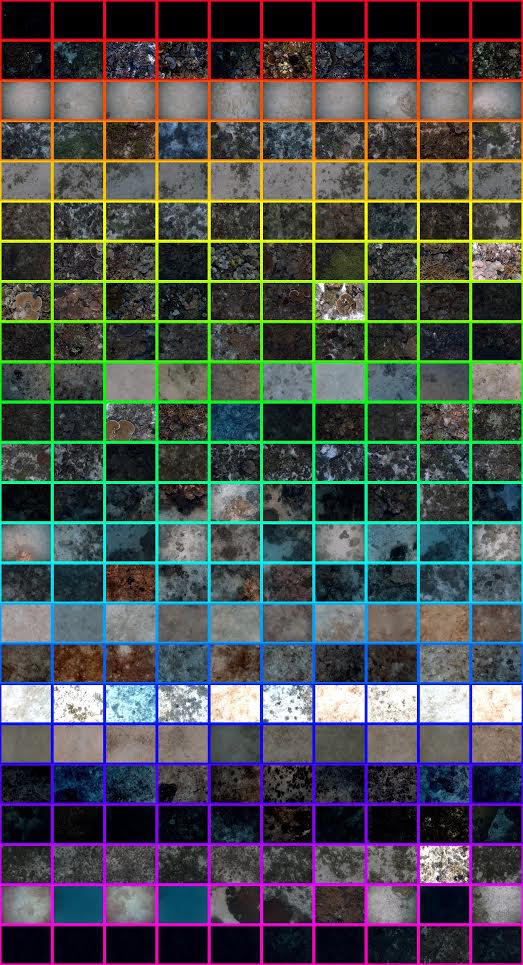
\includegraphics[width=\linewidth]{Figures/label_images.png}
			\caption{Gaussian LDA \\ clustered habitat imagery \\ \citep{Steinberg2015128}}
			\label{Figure:LabelImages}
		\end{wrapfigure}
			
		With the bathymetric depth recorded at both training locations $P$ and query locations $P^{\star}$, the corresponding bathymetric features $X$ and $X^{\star}$ can be extracted through the process detailed in section \ref{BenthicHabitatMapping:BathymetricFeatures}. Along with the benthic habitat labels $\bvec{y}$ observed at the training points, the effective dataset consists of the training data $(P, X, \bvec{y})$ and query data $(P^{\star}, X^{\star})$.

		The habitat labels are clustered in an unsupervised manner from the collected benthic imagery using Gaussian latent Dirichlet allocation (LDA) \citep{Steinberg2015128}, producing 24 unique benthic class labels, with 17 of them associated with identifiable semantic meaning and the rest either over-exposed or under-exposed in lighting (figure \ref{Figure:LabelImages}). For example, the first two rows in Figure \ref{Figure:LabelImages} are under-exposed and thus will not be included in the analysis. Therefore, benthic habitat mapping over Scott Reef is a multiclass classification problem with $n_{C} = 17$ classes.
		
		As discussed in section \ref{BenthicHabitatMapping:BathymetricFeatures}, the benthic habitats are to be modelled upon five bathymetric features - bathymetric depth, aspect (short scale), rugosity (short scale), aspect (long scale), and rugosity (long scale). The corresponding feature maps across the reef have been visualised in Figure \ref{Figure:ScottReefBathymetricFeatures}.
			
		For the Scott Reef dataset, an OVA Gaussian process classifier is employed due to its simpler structure and stronger inference capabilities under \textit{relatively} small training datasets. While the training dataset is large in size, it is \textit{relatively} small compared to the total region to be mapped. As before, the classifier is trained under Laplace approximation as a good balance between tractability and accuracy. The probit response is chosen as the likelihood response, and the kernel covariance employed is an axis aligned squared exponential kernel.
			
		\subsection{Problems and Solutions to Big Data}
		\label{BenthicHabitatMapping:ScottReef:BigData}
		
			One of the problems of performing inference on big datasets is that it has high memory and time complexity requirements. In the current Scott Reef example, there are a total of $n = 34890$ training points and $n^{\star} = 17675180$ query points, even after removing all invalid entries. With regards to the training stage, since Gaussian processes are $O(n^{3})$ algorithms, the high number of training points will cause learning bottlenecks in the process.
			
			More importantly, however, is the memory requirements involved in the inference stage. As explained in sections \ref{Background:GaussianProcesses:Regression} and \ref{BenthicHabitatMapping:Classification}, the inference stage requires the computation of a data kernel $K \in \mathbb{R}^{n \times n}$, an inference kernel $K^{\star} \in \mathbb{R}^{n \times n^{\star}}$, and a query kernel $K^{\star \star} \in \mathbb{R}^{n^{\star} \times n^{\star}}$. Since $n^{\star}$ is orders of magnitude greater than $n$, the memory requirements are dominated by $K^{\star \star}$. Fortunately, in the mapping scenario, it is not necessary to know the covariances between all the query points. Merely the variances at each query point needs to be known such that only the diagonal elements of $K^{\star \star}$ is required, which is $n^{\star}$ in length. The details of this computational shortcut is detailed in appendix \ref{Appendix:ComputationalAspects:TimeSpaceComplexity:CovarianceAvoidance}. However, the full inference kernel $K^{\star}$ is required in order to relate the training points to the query points, without which no inference can be performed. The inference kernel has $n \times n^{\star} = 616687030200 \approx 6 \times 10^{11}$ elements. Even if 32 bit floats instead of 64 bit floats are used, each element takes 32 bits = 4 bytes of memory, such that the total memory requirement for the inference kernel using the entire dataset would be $616687030200 \times 4$ bytes $\approx 2297$ GB \textit{for each binary classifier}. With an OVA classifier for 17 labels, this means more than 39 TB of storage is needed, which is infeasible to store on a standard computer of 4 to 16 GB RAM.
			
			As such, it is imperative to perform analysis with a sample of the dataset. As this section also serves to demonstrate the situation before a path planning mission is initiated, small numbers of training points will be chosen to reflect the high uncertainty in the resulting map due to a lack of data. In the following sections, $n = 200$ training points and $n^{\star} = 100000$ query points are randomly selected from the dataset for map inference, which forms the effective training data $(P, X, \bvec{y})$ and query data $(P^{\star}, X^{\star})$.
			
		\subsection{Prediction Map}
		\label{BenthicHabitatMapping:ScottReef:Maps}

			As training labels are only available around past mission tracks (figure \ref{Figure:ScottReefBathymetricFeatures:1}), a synthetic ground truth is generated separately in order to assess the mapping performance (figure \ref{Figure:ScottReefSyntheticGroundTruth}). Only the 17 labels out of the 22 image clusters that are identifiable are shown. This ground truth is generated separately with 800 training points available in the dataset, which is a reasonable size on a computer with 8 GB RAM as the inference kernel would take $800 \times 100000 \times 17 \times 4$ bytes $\approx 5$ GB of storage. Since the synthetic ground truth is generated with only 800 training points, it does not necessary represent the physical reality at Scott Reef. 
	
			\begin{figure}[!htbp]
			\centering
				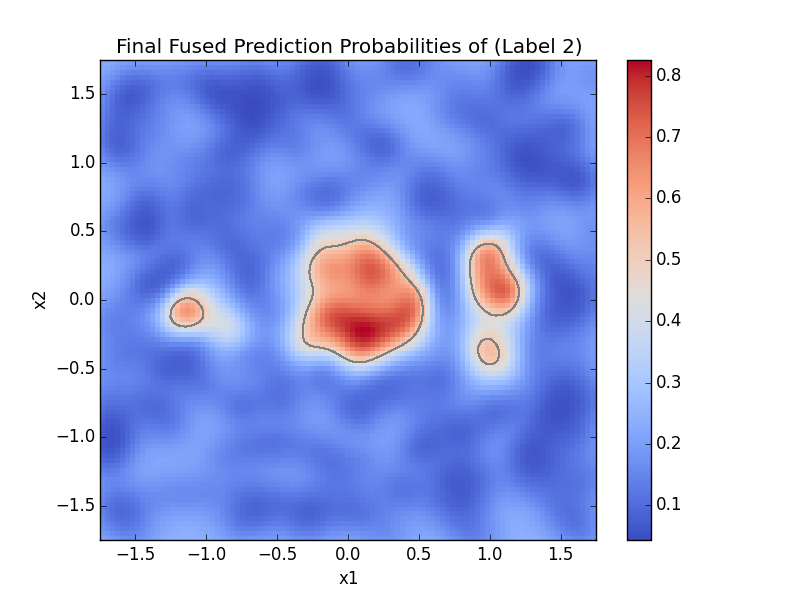
\includegraphics[width = 0.8\linewidth]{Figures/scott_reef_mapping/Figure7.eps}
			\caption{Scott Reef: Synthetic Ground Truth}
			\label{Figure:ScottReefSyntheticGroundTruth}
			\end{figure}
			
			With merely 200 training points, the classifier is able to infer a map which achieves a 41.54\% misclassification rate, or 58.46\% prediction accuracy, over 100000 query points (figure \ref{Figure:ScottReefInitialPredictions200}). This demonstrates the advantage of modeling the benthic environment upon a bathymetric feature space instead of spatial coordinates. The training tracks covers $\frac{200}{100000} = 0.2\%$ of the query region, yet almost 60\% of the region can be accurately modeled with such scarce data. This model takes advantage of the fact that although habitats can be far away spatially, they can have similar bathymetric structures such that they are close in the bathymetric feature space.
			
			\begin{figure}[!htbp]
			\centering
			  \subfigure[Initial Prediction with 200 training points]{\label{Figure:ScottReefInitialPredictions200}	\includegraphics[width=0.8\linewidth]{Figures/scott_reef_mapping/Figure8.eps}}
			  \subfigure[Initial Prediction with 400 training points]{\label{Figure:ScottReefInitialPredictions400}	\includegraphics[width=0.48\linewidth]{Figures/scott_reef_mapping_400/Figure8.eps}}
			  \subfigure[Initial Prediction with 600 training points]{\label{Figure:ScottReefInitialPredictions600}	\includegraphics[width=0.48\linewidth]{Figures/scott_reef_mapping_600/Figure8.eps}}
			\caption{Scott Reef: Initial Predictions}
			\label{Figure:ScottReefInitialPredictions}
			\end{figure}

			The effect of increasing the number of randomly selected training points from the training data set is shown in Figure \ref{Figure:ScottReefBathymetricFeatures:1}. As subsequently added training points are still within similar regions with similar bathymetric signatures, the classification accuracy does not necessarily improve.
												
	\section{Summary}
	
			